\chapter{Revisão Bibliográfica}

Este capítulo de revisão bibliográfica está estruturado em quatro seções principais que contextualizam os objetivos do presente trabalho. A seção \ref{sec:Fofos} fornece uma descrição, com enfoque nas transformações de fases, do atual conhecimento sobre o material estudado neste trabalho, o ferro fundido nodular. Nesta seção também são apresentados dois importantes assuntos utilizados na discussão dos resultados deste trabalho, a microsegregação de elementos de liga durante a solidificação do metal e a interrupção da reação bainítica para produção de microestruturas compostas de ferrita e austenita estabilizada por enriquecimento em carbono.

Na seção \ref{sec:consTransf} são expostos conceitos sobre controle cinético de transformações difusionais, utilizados no modelo termodinâmico para predição das microestruturas produzidas pelo processo de Têmpera e Partição (T\&P). Na seção seguinte, é apresentada uma descrição sobre a transformação martensítica em ligas ferrosas baseada no entendimento consolidado sobre esta reação. Procurou-se omitir aspectos sobre a cristalografia da transformação e a discussão sobre o mecanismo da reação bainítica, ainda alvo de controvérsia.

Por fim, na seção \ref{sec:processoTP} é apresentada a revisão bibliográfica sobre o processo de Têmpera e Partição, enfatizando os trabalhos exploratórios do grupo da \enfase{Colorado School of Mines} no início da década de 2000 e o modelo termodinâmico desenvolvido por Speer e colaboradores \cite{Speer2003}. Também foi incluída nesta seção uma revisão sobre transformações que podem ocorrer competitivamente durante a etapa de partição do processo T\&P.

\section{Ferros fundidos nodulares}

\label{sec:Fofos}

Os ferros fundidos, de forma simplificada, podem ser considerados ligas ternárias Fe-C-Si, contendo também teores de impurezas (Mn, P e S) e de elementos adicionados intencionalmente como agentes modificadores (Mg e Ce). Sua solidificação apresenta uma fase pró-eutética (austenita ou grafita), completada por uma reação de solidificação eutética, que pode ser estável ($\text{líquido} \rightarrow \text{austenita} + \text{grafita}$), ou metaestável ($\text{líquido} \rightarrow \text{austenita} + \text{cementita}$).

Ferros fundidos nodulares correspondem a uma classe dos ferros fundidos em que a morfologia da grafita é apresentada na forma de nódulos esferoidizados, estrutura conseguida por meio da adição de elementos químicos modificadores, sendo o Mg e o Ce os mais comuns.

A grafita é formada pelo empilhamento de camadas planas constituídas de átomos de carbono ligados covalentemente na forma de uma estrutura hexagonal. Durante a solidificação, a grafita pode crescer na direção dos planos basais ou dos planos prismáticos (vide figura \ref{fig:grafita}), assumindo a forma de lamelas ou esferas em função da composição química e do processamento do metal líquido. Elementos tensoativos, como oxigênio e enxofre, tendem a ser adsorvidos pelos planos prismáticos da célula da grafita, diminuindo a energia interfacial destas superfícies e, portanto, favorecendo o crescimento da fase nestas direções, resultando em morfologias lamelares. Na ausência destas impurezas, o crescimento nos planos prismáticos não é favorecido e, em consequência, a grafita preponderantemente na direção dos planos basais, adquirindo a morfologia de glóbulos esféricos. A utilização de magnésio no tratamento pré-vazamento do metal líquido visa a eliminação das impurezas e a obtenção de grafita nodular, uma vez que o Mg possui forte ação desoxidante e dessulfurante\cite{Labrecque1998,Guesser2009}.

\begin{figure}
	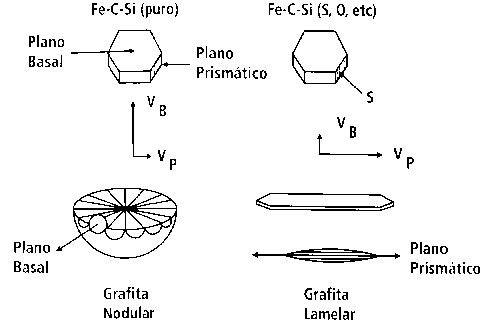
\includegraphics[width=10cm]{img/grafita.pdf}
	\caption{Esquema de crescimento da grafita nas direções normais aos planos basais e prismáticos\cite{Guesser2009}.}
	\label{fig:grafita}
\end{figure}

É comum a prática de inoculação do ferro fundido com elementos de ação grafitizante, pouco antes de seu vazamento, com o objetivo diminuir o super-resfriamento para o início da formação da grafita e, assim, evitar que o eutético metaestável seja formado\cite{Santos1991}. O grau de inoculação de ferros fundidos nodulares controla a dispersão dos nódulos de grafita no metal e, consequentemente, também o espaçamento entre as células eutéticas.

\subsection{Solidifica\c{c}\~{a}o}

A solidificação dos ferros fundidos nodulares é descrita de acordo com as reações dos eutéticos estável $\text{líquido} \rightarrow \text{austenita} + \text{grafita}$. A composição química e a velocidade de resfriamento são os principais parâmetros que definem a natureza da reação eutética nos ferros fundidos. Enquanto no sistema Fe-C a diferença entre as temperaturas de equilíbrio do eutético estável e metaestável é de aproximadamente 7 °C, ligas contendo 2\% em massa de silício tem essa faixa ampliada para 35 °C\cite{Santos1991}. O silício e outros elementos que possuem a propriedade de aumentar a diferença entre os dois eutéticos, como o alumínio, níquel e cobre, são chamados de elementos grafitizantes. Por outro lado, elementos que são fortes formadores de carbonetos, como o cromo, vanádio e o tungstênio tendem a aproximar os dois eutéticos. Por esta propriedade, são geralmente empregados na produção de ferros fundidos brancos. Altas taxas de resfriamento favorecem a formação do eutético metaestável, uma vez que a formação da cementita é mais rápida do que a precipitação da grafita.

Em ferros nodulares de composição eutética, a solidificação se inicia após a aplicação de um super-resfria-%atentar a essa quebra de linha
mento ao líquido a temperaturas inferiores à do eutético estável, quando se dá a nucleação e crescimento dos nódulos de grafita. Na sequência, os nódulos formados são encapsulados por um invólucro de austenita, formando a denominada célula eutética. As células eutéticas continuam crescendo até que todo o calor latente da solidificação seja liberado e a solidificação tenha chegado a seu fim\cite{Santos1991}. %Vide\cite{Stefanescu2005} para citar Patterson e Scheil (1949)

A reação eutética no ferro fundido nodular apresenta uma característica que o difere, por exemplo, da reação eutética em um ferro fundido cinzento. Neste último caso, os dois produtos da reação, austenita e grafita de morfologia lamelar, se formam simultaneamente. No ferro fundido nodular a formação da austenita e da grafita ocorre em momentos distintos. O constituinte eutético é, portanto, do tipo ``divorciado'', em contraste ao crescimento cooperativo observado na reação eutética de ferros cinzentos\cite{Santos1991}.

Em ligas hipoeutéticas e hipereutéticas, por sua vez, há a formação de uma fase primária no início da solidificação. No primeiro caso, a solidificação se inicia com a formação de dendritas de austenita, enquanto no segundo caso nódulos de grafita são formados diretamente a partir do líquido. Em ambos os casos, na medida em que o material é resfriado, a composição do líquido progressivamente se aproxima da composição eutética. A reação eutética, no entanto, só se inicia uma vez atingido um super-resfriamento suficiente para nucleação e crescimento dos nódulos de grafita\cite{Santos1991}.

Na microestrutura final das ligas eutética e hipoeutética é normalmente observada uma população de nódulos de grafita com tamanhos dispersos segundo uma distribuição Gaussiana. Em ligas hipereutéticas, por sua vez, são observadas duas diferentes populações de nódulos de grafita: uma cuja média dos diâmetros é maior, correspondente aos nódulos formados entre a temperatura \enfase{liquidus} e a temperatura do eutético metaestável, e outra cujo tamanho médio da população é menor, formada durante a reação eutética\cite{Santos1991}. %citar quem o Santos cita

\subsubsection{Microsegrega\c{c}\~{a}o de elementos durante a solidifica\c{c}\~{a}o}

Microsegregação é o termo que define a condição de não-uniformidade de composição química no material a nível microestrutural. Em complemento à definição de microsegregação, macrosegregação trata-se da não-uniformidade de composição química em larga escala, comparável ao tamanho da peça. A macrosegregação é um defeito do processo de fundição do metal e, portanto, seu controle possui caráter tecnológico. Por outro lado, a microsegregação é inerente ao produto fundido e, dessa forma, tem sua devida importância reconhecida nesta seção do texto.

A microsegregação se origina devido à expulsão de soluto da fase sólida ao crescer a partir do metal líquido. Caso a liga seja resfriada lentamente, o contato prolongado entre líquido e sólido permitirá a difusão de soluto até o estabelecimento do equilíbrio termodinâmico para cada temperatura; esta construção hipotética leva à elaboração dos diagramas de fase. No entanto, nas situações reais, em que taxas de resfriamento elevadas são impostas ao material, a rejeição do soluto da fase sólida para a fase líquida estabelece uma heterogeneidade de composição ao final da solidificação. Dessa forma, na microestrutura bruta de fundição há a preponderância do soluto nas últimas porções de metal a se solidificar.

Em ferros fundidos a microsegregação também é originada na formação da fase de solidificação primária, mas é principalmente atribuída à reação eutética. Como estas ligas possuem ao menos três elementos químicos, a regra das fases de Gibbs\footnotemark prevê que a reação eutética $\text{líquido} \rightarrow \text{austenita} + \text{grafita}$ não ocorre em um ponto invariante, mas sim em uma faixa de temperaturas. Devido às limitadas difusividades dos elementos na fase sólida e à dependência de suas solubilidades no líquido em função da temperatura de solidificação, ocorre que as sucessivas camadas de austenita formadas a partir do líquido apresentam diferentes composições químicas. Assim, elementos que apresentam maior solubilidade na austenita em temperaturas mais elevadas, como silício, níquel e cobre, tendem a se concentrar nas primeiras regiões a se solidificar. Na formação do eutético divorciado do ferro nodular, portanto, estes elementos se concentrarem próximos aos nódulos de grafita. Por outro lado, carbono, enxofre, manganês, cromo e molibdênio são rejeitados da austenita para líquido e acabam permanecendo em maior concentração nas últimas regiões a se solidificar, isto é, aquelas que correspondem ao encontro das células eutéticas. %Referenciar e inserir figura

\footnotetext{A regra das fases foi proposta por J.W. Gibbs em seu famoso trabalho de 1878 \enfase{On the Equilibrium of Heterogeneous Substances}\cite{Gibbs1878}. A equação estabelece a igualdade $F = C - P + 2$, em que $F$ é o número de graus de liberdade (número de variáveis de estado independentes), $C$ o número de componentes do sistema e $P$ o número de fases. Para um sistema constituído apenas de fases condensadas, em que o efeito da pressão é desprezível, pode ser simplificado para $F = C - P + 1$.}

Uma ferramenta muito útil para o entendimento e quantificação (estimativa) da microsegregação é o modelo de Scheil-Gulliver. %\cite{Porter2009}
A equação desenvolvida por Scheil apud \citaremsentenca{Porter2009} %pegar referência original do Scheil?
vale para uma liga binária cuja solidificação gera apenas uma fase sólida. As hipóteses de Scheil representam a situação de máxima segregação, em que a difusão do soluto na fase sólida é completamente desprezada e, portanto, não é possível o estabelecimento do equilíbrio termodinâmico em todo o sistema. As considerações feitas neste modelo são\cite{Porter2009}:

\begin{enumerate}
	\item Não há difusão na fase sólida após sua formação;
	\item A difusão é infinitamente rápida na fase líquida para todas as temperaturas. Essa ponderação é equivalente a considerar a composição química homogênea ao longo de todo o líquido;
	\item As composições na interface sólido-líquido são de equilíbrio, valendo as composições preditas pelo diagrama de fases em uma dada temperatura. Essa hipótese não significa que há o estabelecimento do equilíbrio no sistema, mas \enfase{apenas} na interface. Ela é semelhante à adotada por Zener para transformações difusionais em estado sólido (vide seção \ref{sec:consTransf});
	\item As linhas \enfase{solidus} e \enfase{liquidus} são representadas por linhas retas no diagrama de fases. \label{item:scheil4}
\end{enumerate}

Postas estas condições, define-se o coeficiente de partição $k$, que corresponde à razão entre o teor de soluto $C_S$ na fase sólida a composição química $C_L$ na fase líquida, ambas consultadas no diagrama de fases:

\begin{subequations}
	\begin{align}
		\label{eq:coefPart}k = \frac{C_S}{C_L}
	\end{align}
\end{subequations}

Note-se que, devido à hipótese \ref{item:scheil4}, $k$ assume valor constante. Atualmente, graças ao aumento do poder computacional e ao desenvolvimento de bases de dados termodinâmicos, esta hipótese pode ser relaxada utilizando técnicas numéricas, tais quais as empregadas nos pacotes de software que empregam o método CALPHAD. %pacote de software? protocolo? não sei direito o que é o CALPHAD

\novasiglaestrangeira{CALPHAD}{Computer Coupling of Phase Diagrams and Thermochemistry} %Prestar atenção se fica dentro ou fora da ordem alfabética.

As demais equações que definem o problema consistem da condição inicial de solidificação (equação \ref{eq:condIni}), isto é, que a composição do líquido no início da solidificação é igual à composição média da liga $C_0$, a conservação de massa do sistema (equação \ref{eq:balSis}), dada pela soma unitária das frações de sólido ($f_S$) e líquido ($f_L$), e o balanço de massa na interface (equação \ref{eq:Stefan}), que corresponde ao balanço entre a redistribuição do soluto e o aumento da fração de sólido.

\begin{subequations}[resume]
	\begin{align}
		\label{eq:condIni}\left.C_L\right|_{f_S=0} &= C_0\\
		\label{eq:balSis}f_S + f_L &= 1\\
		\label{eq:Stefan}\left(C_L - C_S\right) df_S &= f_L dC_L
	\end{align}
\end{subequations}

A integração da equação diferencial \ref{eq:Stefan} nos domínios de integração definidos pela condição inicial (equação \ref{eq:condIni}) utilizando as substituições dos termos adequados obtidos pelas equações \ref{eq:coefPart} e \ref{eq:balSis} leva à equação de Scheil-Gulliver para composição do sólido e do líquido durante a solidificação:

\begin{subequations}
	\begin{align}
		C_L &= C_0 {f_L}^{k-1}\\
		\label{eq:C_S}C_S &= k C_0\left(1 - f_S\right)^{k-1}
	\end{align}
\end{subequations}

Graças ao desenvolvimento de bases de dados termodinâmicas é possível também utilizar as considerações de Scheil para estimar a microsegregação durante a solidificação de ligas multicomponentes, que frequentemente geram mais de uma fase sólida diretamente do líquido. Softwares que seguem o método CALPHAD, como o Thermo-Calc\textregistered, possuem módulos que permitem esse tipo de contabilização. Adicionalmente, quando acoplados com informações sobre a difusividade dos elementos químicos, também permitem a utilização de condições de equilíbrio parcial na interface (tal quais as apresentadas na seção \ref{sec:consTransf}) e aplicação de difusão no estado sólido\cite{Chen2002,Larouche2007}.

\subsection{Transforma\c{c}\~{o}es no estado s\'{o}lido}

Durante o resfriamento lento do metal solidificado, em torno de 720 °C ocorre a decomposição eutetóide da austenita, que, assim como a reação eutética, pode acontecer na forma estável ($\text{austenita} \rightarrow \text{ferrita} + \text{grafita}$) ou metaestável ($\text{austenita} \rightarrow \text{ferrita} + \text{cementita}$). A predominância de uma reação ou outra é novamente dependente da taxa de resfriamento e da composição química.

Durante a reação do eutetóide estável, a austenita se decompõe em ferrita e grafita secundária. A nucleação da ferrita se dá preferencialmente na interface entre a austenita e os nódulos de grafita formados durante a solidificação. A ferrita cresce para o interior da austenita, enquanto a grafita é incorporada aos nódulos pré-existentes. Em estágios avançados da reação a ferrita engloba completamente o nódulo, formando uma barreira para a difusão de carbono da austenita para a grafita, diminuindo substancialmente a velocidade da reação. A tendência a partir desse ponto é que a reação do eutetóide metaestável, que corresponde à decomposição da austenita em perlita, predomine e consuma a austenita não-transformada. A figura \ref{matrizFofo} ilustra a sequência de etapas da decomposição eutetóide da austenita.

\begin{figure}
	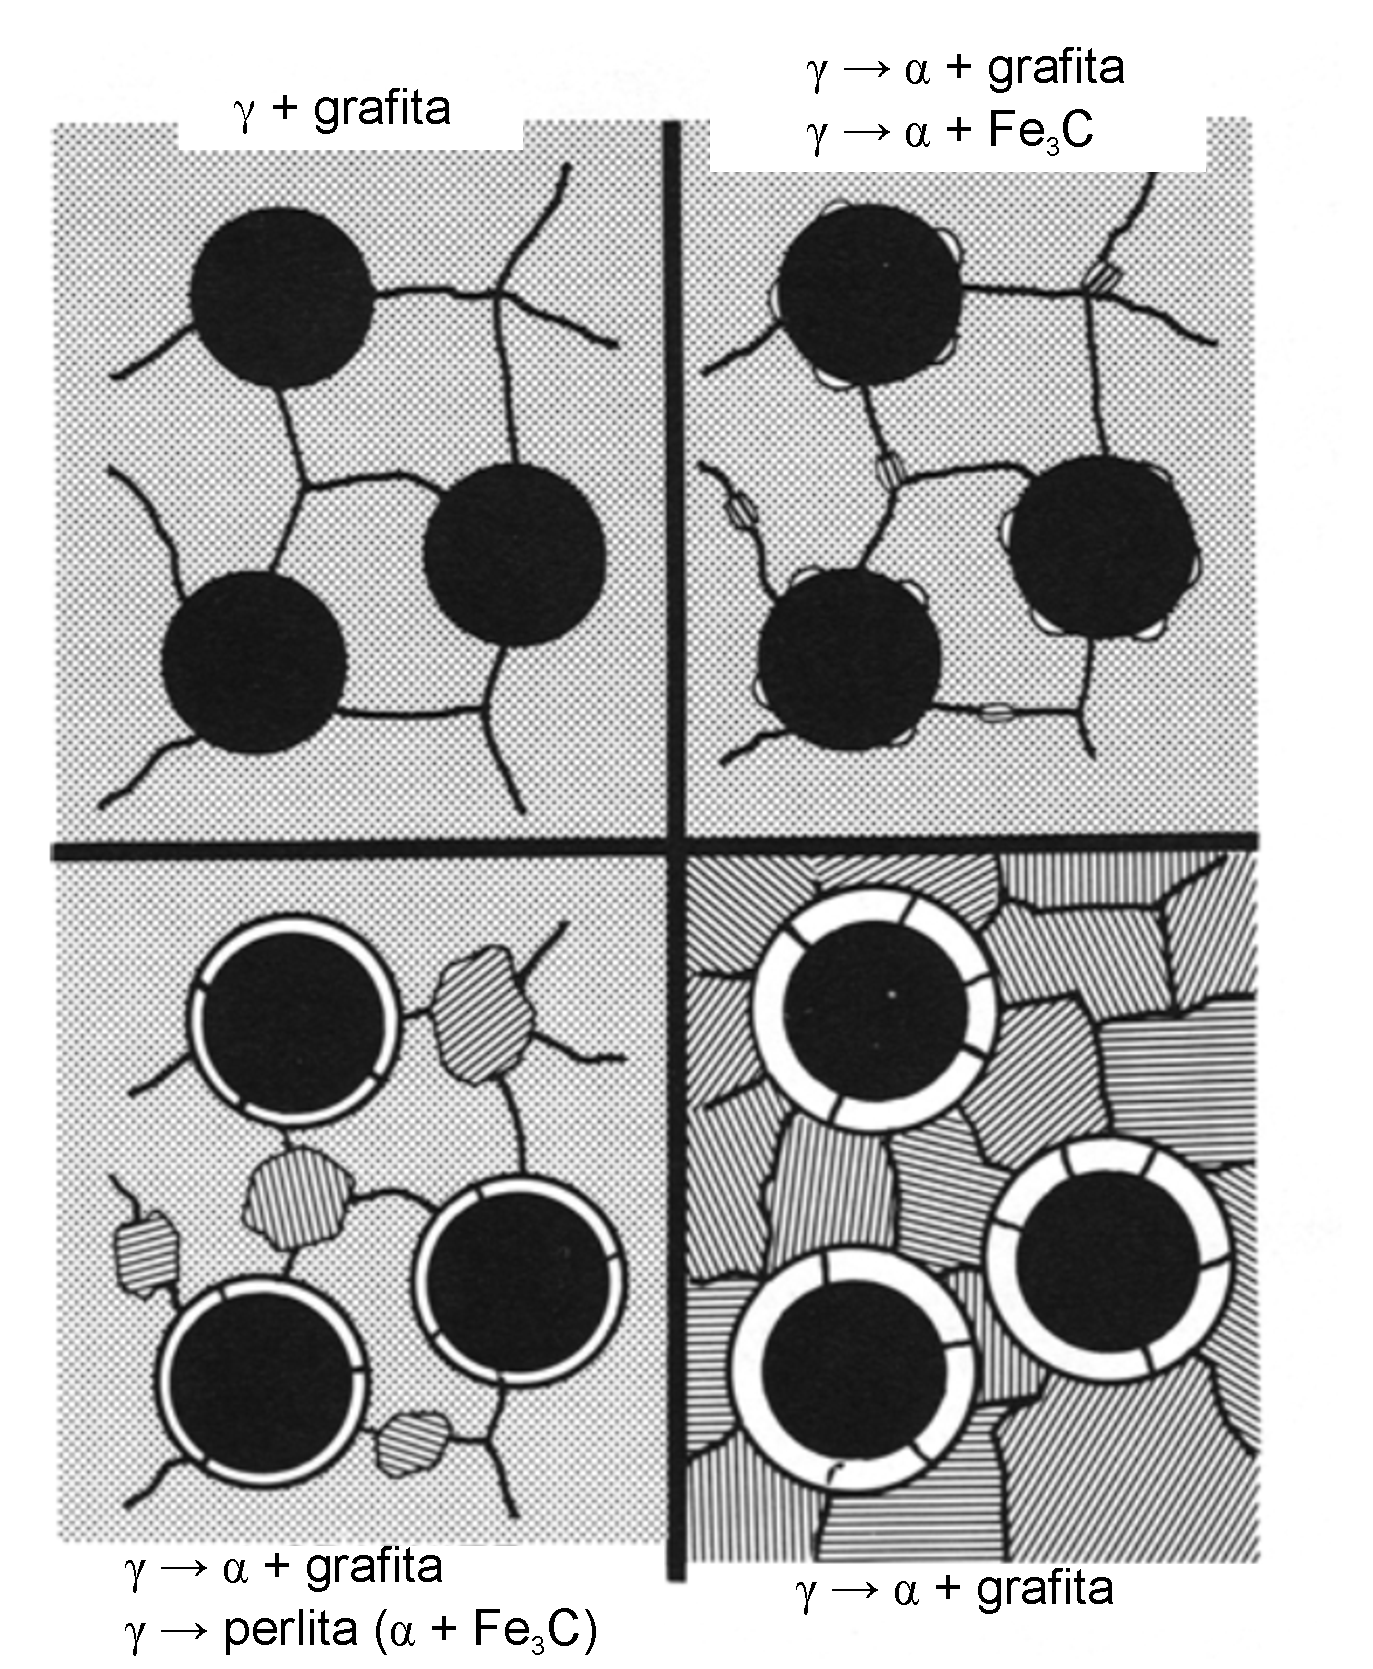
\includegraphics[width=10cm]{img/matrizFofo.pdf}
	\caption{Ilustração esquematizando a decomposição eutetóide em ferros fundidos nodulares\cite{Johnson1978}.}
	\label{matrizFofo}
\end{figure}

A perlita consiste de um agregado de lamelas alternadas de ferrita e cementita. O crescimento da perlita se dá de forma cooperativa, ou seja, as duas fases crescem simultaneamente. Ao contrário da precipitação de grafita no estado sólido, a formação de cementita não carece da difusão a longo alcance dos átomos de Fe. Por este motivo, para uma ampla faixa de temperaturas a cinética da reação perlítica é consideravelmente mais rápida do que a formação do eutetóide estável. \citaremsentenca{Zener1946} estudou a cinética local de crescimento da perlita assumindo que a distância de difusão característica de seu crescimento seria o espaçamento interlamelar. Em consequência, Zener concluiu que a velocidade de crescimento de uma colônia é constante e independente da porção transformada da austenita, ao contrário do que acontece no eutetóide estável.

Elementos como antimônio, cobre e estanho são chamados de ``perlitizantes'' por atuarem evitando a formação da ferrita oriunda do eutetóide estável\cite{Kovacs1981}.
A obtenção de uma matriz perlítica também pode ser conseguida por meio de tratamentos térmicos, como é o caso da normalização. Matrizes completamente ferríticas também podem ser obtidas por meio tratamentos térmicos. O recozimento é um tratamento térmico em que a peça é aquecida a temperaturas próximas à de início de eutetóide estável que leva à dissociação da perlita para formação da estrutura de equilíbrio ferrita + grafita\cite{Guesser2009}.

Além das matrizes ferrítica e perlítica convencionais, ferros fundidos podem ser submetidos a tratamentos de têmpera, para obtenção de uma matriz martensítica, e austêmpera, para obtenção de matriz constituída de bainita isenta de carbonetos e austenita retida estabilizada por carbono. Estas matrizes conferem ao material resistência mecânica muito superiores às matrizes ferrítica e perlítica e, no caso do produto austemperado, elevadas ductilidade e tenacidade ao impacto\cite{Guesser2009}.

\subsection{Ferro fundido nodular austemperado (ADI)}

\label{subsec:ADI}

Em aços carbono, tratamentos isotérmicos aplicados à austenita em temperaturas inferiores às de formação da perlita geram um microconstituinte eutetóide denominado bainita. Morfologicamente, a bainita se apresenta na forma de ripas de ferrita (ou agulhas, como é visto em uma seção bidimensional) contendo carbonetos dispersos ou entre cada unidade de ferrita (bainita superior), ou em seu interior (bainita inferior).

Em ligas ferrosas contendo silício a transformação bainítica possui uma cinética característica, consistindo de uma etapa inicial de formação de feixes de ferrita pró-bainítica, prosseguida por um período de estagnação conhecido como ``estase'', para que a reação, enfim, possa ser retomada pela precipitação de carbonetos nas ilhas de austentita não-transformadas\cite{Goldenstein2002}. Durante a primeira etapa da reação nestas ligas, a ferrita bainítica progressivamente enriquece em carbono a austenita adjacente. Como será discutido na seção \ref{sec:Martensita} deste trabalho, austenita com teores elevados carbono possui pouca tendência de se transformar durante o resfriamento. Assim, dependendo do teor médio de carbono da liga, se a reação é interrompida durante a estase, uma grande quantidade de austenita estabilizada em carbono pode ser retida na temperatura ambiente.

O ferro fundido nodular austemperado (do inglês, \siglaestrangeira{ADI}{Austempered Ductile Iron}) faz uso desse fenômeno para obtenção de uma matriz bifásica de finas ripas de ferrita intercaladas com filmes de austenita --- produto chamado de ``ausferrita'' na literatura de fundição. Nos ferros fundidos o fenômeno da estase é prologando devido aos elevados teores de silício inerentes a esse material. Ainda assim, o processo é somente viável em uma ``janela de processo'', que corresponde ao intervalo de tempos e temperaturas em que o produto austemperado confere propriedades dentro das faixas de propriedades estabelecidas pela norma ASTM A897\cite{Bayati1999,ASTMA8972006} e normalmente termina com a precipitação de carbonetos na reação bainítica. Quando produzida nos parâmetros adequados de tratamento térmico, a ausferrita confere ao ADI elevada resistência mecânica aliada a elevada ductilidade devido à ocorrência do efeito TRIP (\enfase{Transformation Induced Plasticity})\cite{Goldenstein2002}. Por este motivo, o ADI proporciona propriedades comparáveis às obtidas em aços, em algumas situações se mostrando favoravelmente competitivo por agregar as vantagens de produção próxima da forma final (\enfase{near-net-shape}) decorrente do processo de fundição\cite{Trudel1997,Hayrynen2002}.

O tratamento térmico para produção do ADI, ilustrado na figura \ref{fig:austempera}, consiste de uma etapa inicial de aquecimento até o campo de equilíbrio entre austenita e grafita (austenitização), na qual o material é mantido durante um determinado tempo de encharque. Em seguida, as peças são mergulhadas em banho de sal fundido, pré-aquecido na temperatura de austêmpera, onde são mantidas por tempo suficiente para que a austenita enriquecida em carbono seja retida à temperatura ambiente\cite{Trudel1997}.

\begin{figure}
	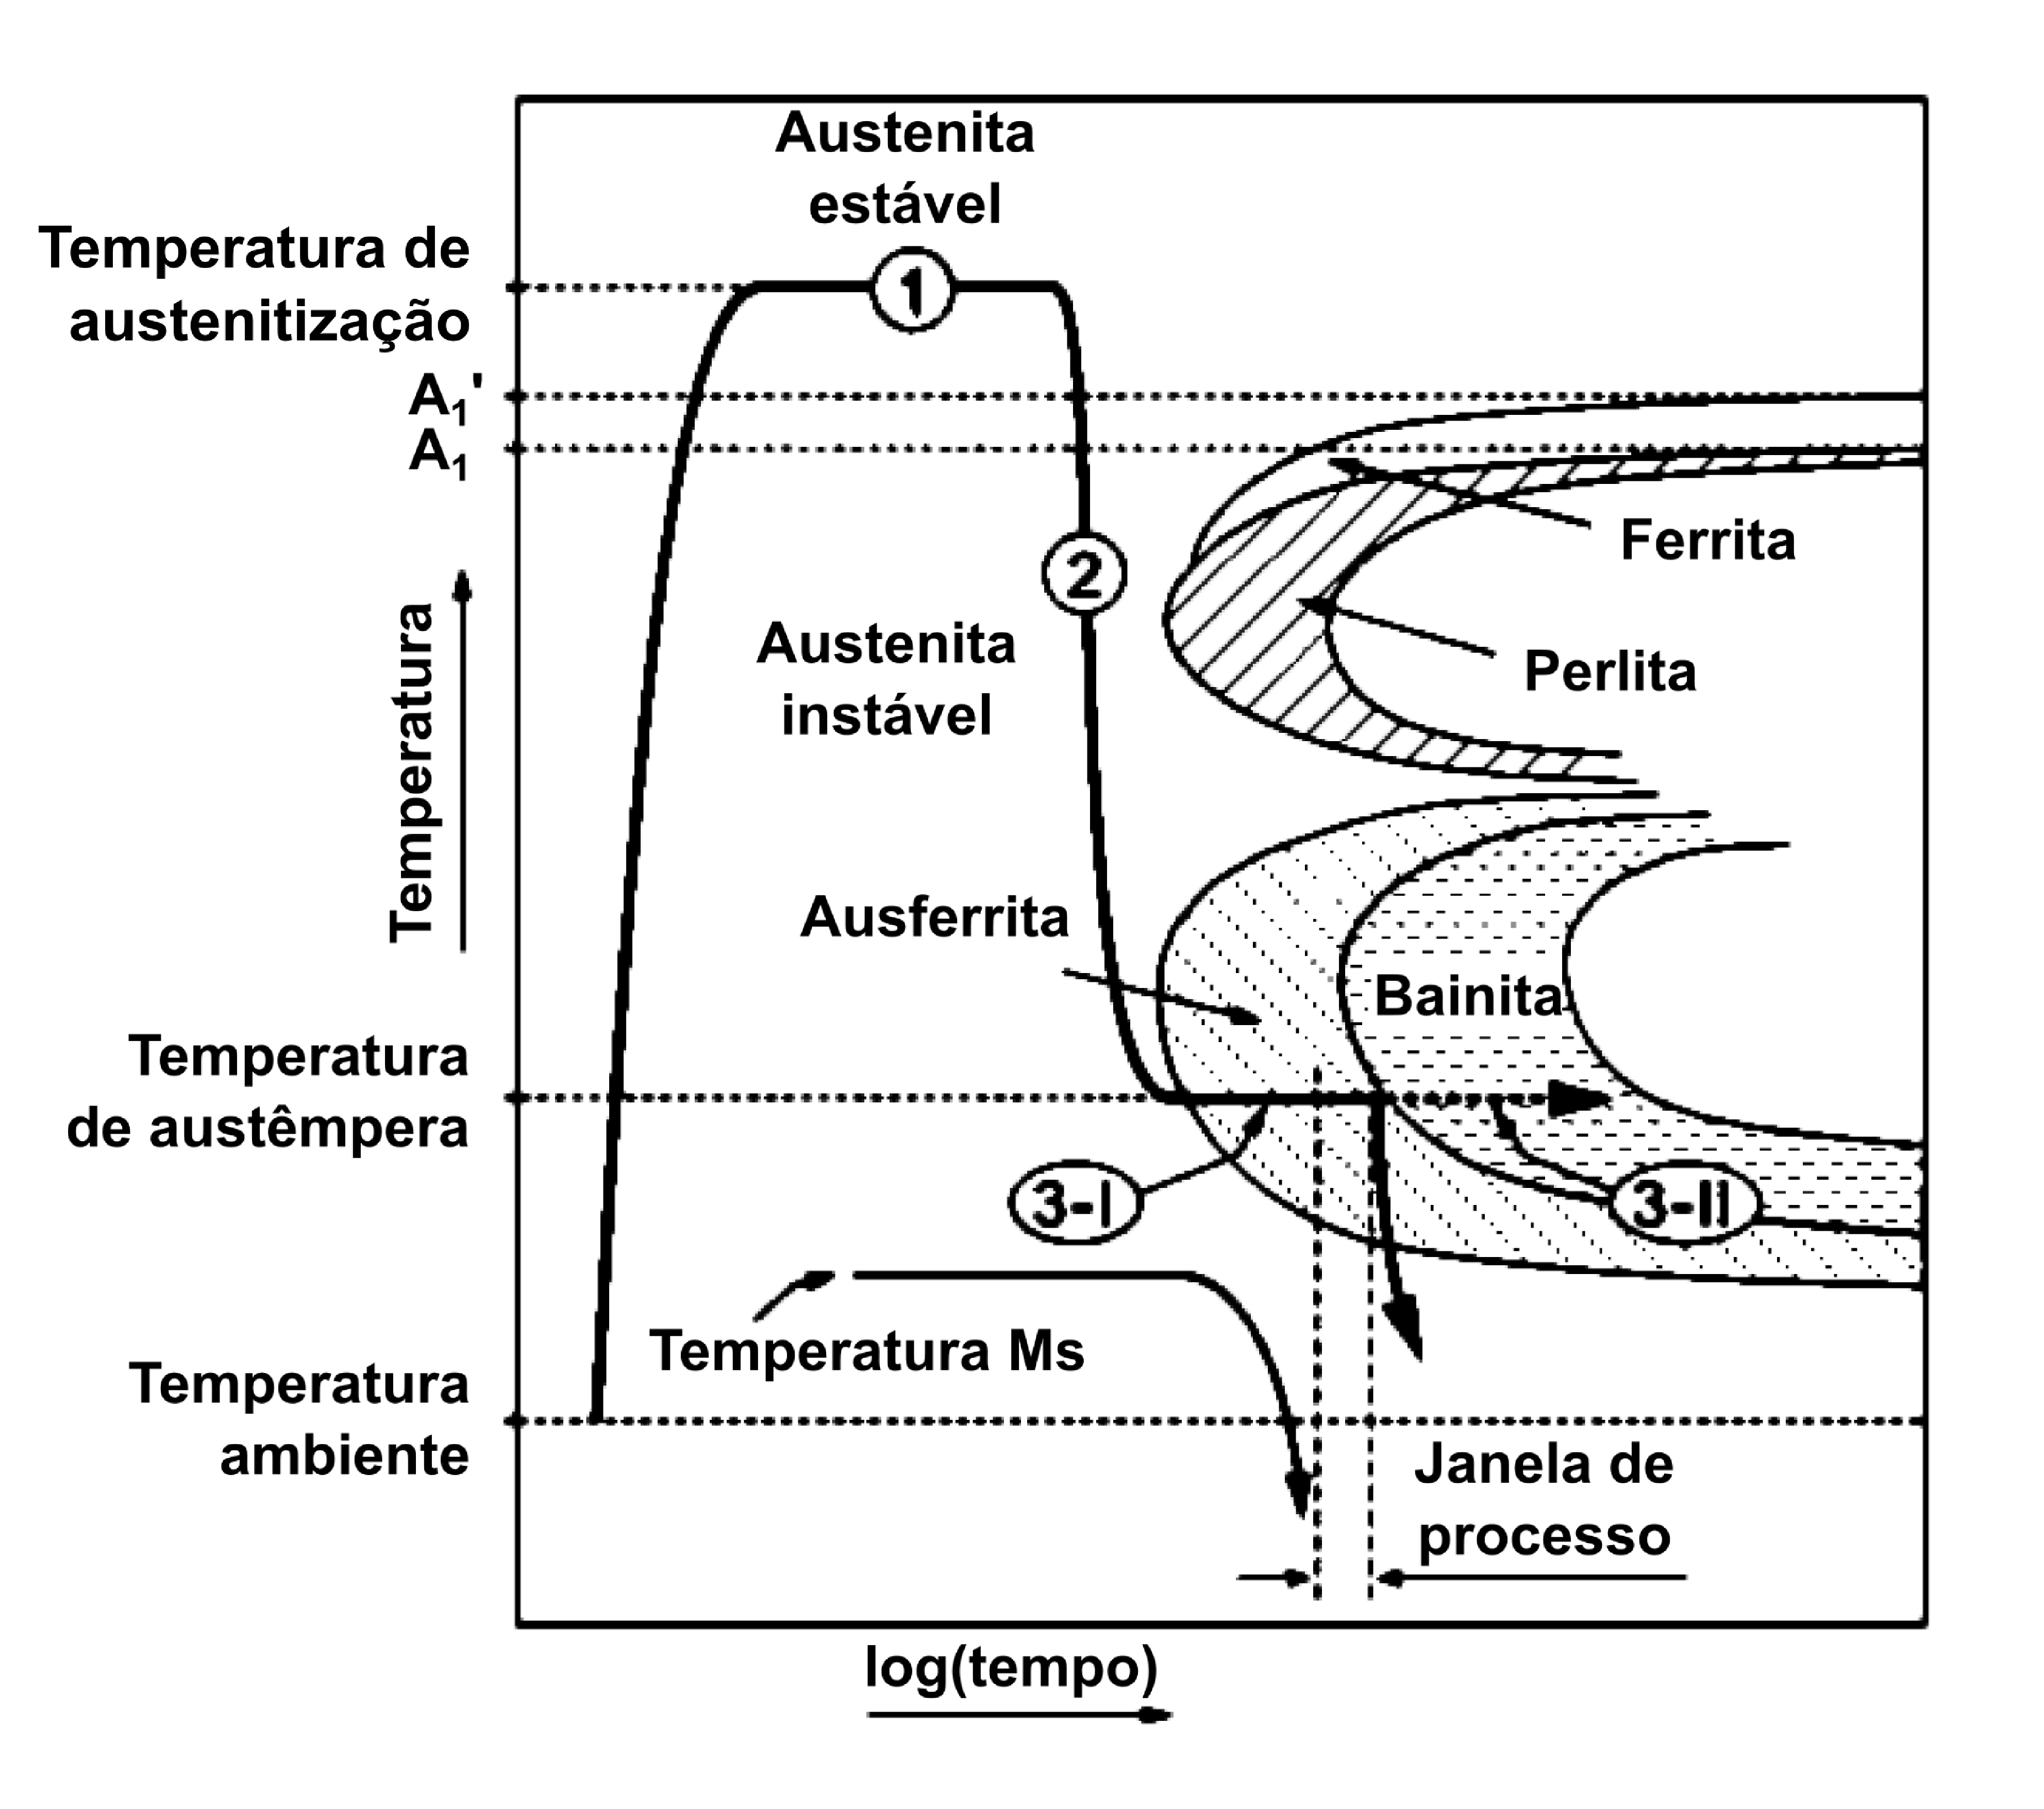
\includegraphics[height=10cm]{img/austemperaTTT_Meier.pdf}
	\caption{Diagrama TTT esquemático ilustrando o processo de austêmpera de ferros fundidos\cite{Meier2013a}.}
	\label{fig:austempera}
\end{figure}

A temperatura de austenitização controla a composição da austenita em equilíbrio com a grafita. Temperaturas mais elevadas ajudam na redistribuição do manganês segregado para os contornos de célula eutética e atribuem um maior teor de carbono à austenita, conferindo, portanto, também maior temperabilidade ao material. Nesse caso, tempos mais prolongados de austêmpera seriam necessários para o início da transformação bainítica e, uma vez estabelecido o final da primeira etapa da reação, maiores frações de austenita retida acabam por ser obtidas. A elevada temperabilidade também confere menor tendência de formação de perlita durante o resfriamento, indesejável para o alcance das propriedades mecânicas\cite{Trudel1997}. O uso intensivo de elementos químicos produz efeito semelhante sobre a temperabilidade do material, mas deve ser utilizado com especial cuidado devido aos problemas associados à microsegregação\cite{Bayati1995,Velez1996}.

\citaremsentenca{Trudel1997} apontam que o tempo de austenitização deve ser o mínimo possível para que garantir que o material se transforme completamente em austenita saturada em carbono e grafita, sendo o tempo de uma hora à temperatura de 900 °C em uma peça de 25 mm de diâmetro geralmente suficiente para garantir isso. No entanto, para temperaturas mais baixas, tempos superiores a três horas podem ser necessários para a eliminação das heterogeneidades de composição química.

A temperatura de austêmpera desempenha o papel mais importante no estabelecimento das propriedades mecânicas do ADI. Temperaturas elevadas levam à formação de um produto com excelente ductilidade e resistência a esforços dinâmicos, enquanto temperaturas baixas geram um produto extremamente resistente e resistência ao desgaste\cite{Lin1996,Aranzabal1997,Magalhaes1998}. Microestruturalmente, a ausferrita formada em duas temperaturas diferentes apresenta mudanças significativas. Como pode ser observado na figura \ref{fig:ADIs}a, o material tratado termicamente a 360 °C apresenta ripas grosseiras de bainita com grandes quantidades de austenita, enquanto ADI produzido a 310 °C possui uma microestrutura mais refinada, composta de menores ilhas de austenita isoladas umas das outras.

\begin{figure}
	\subfloat[]{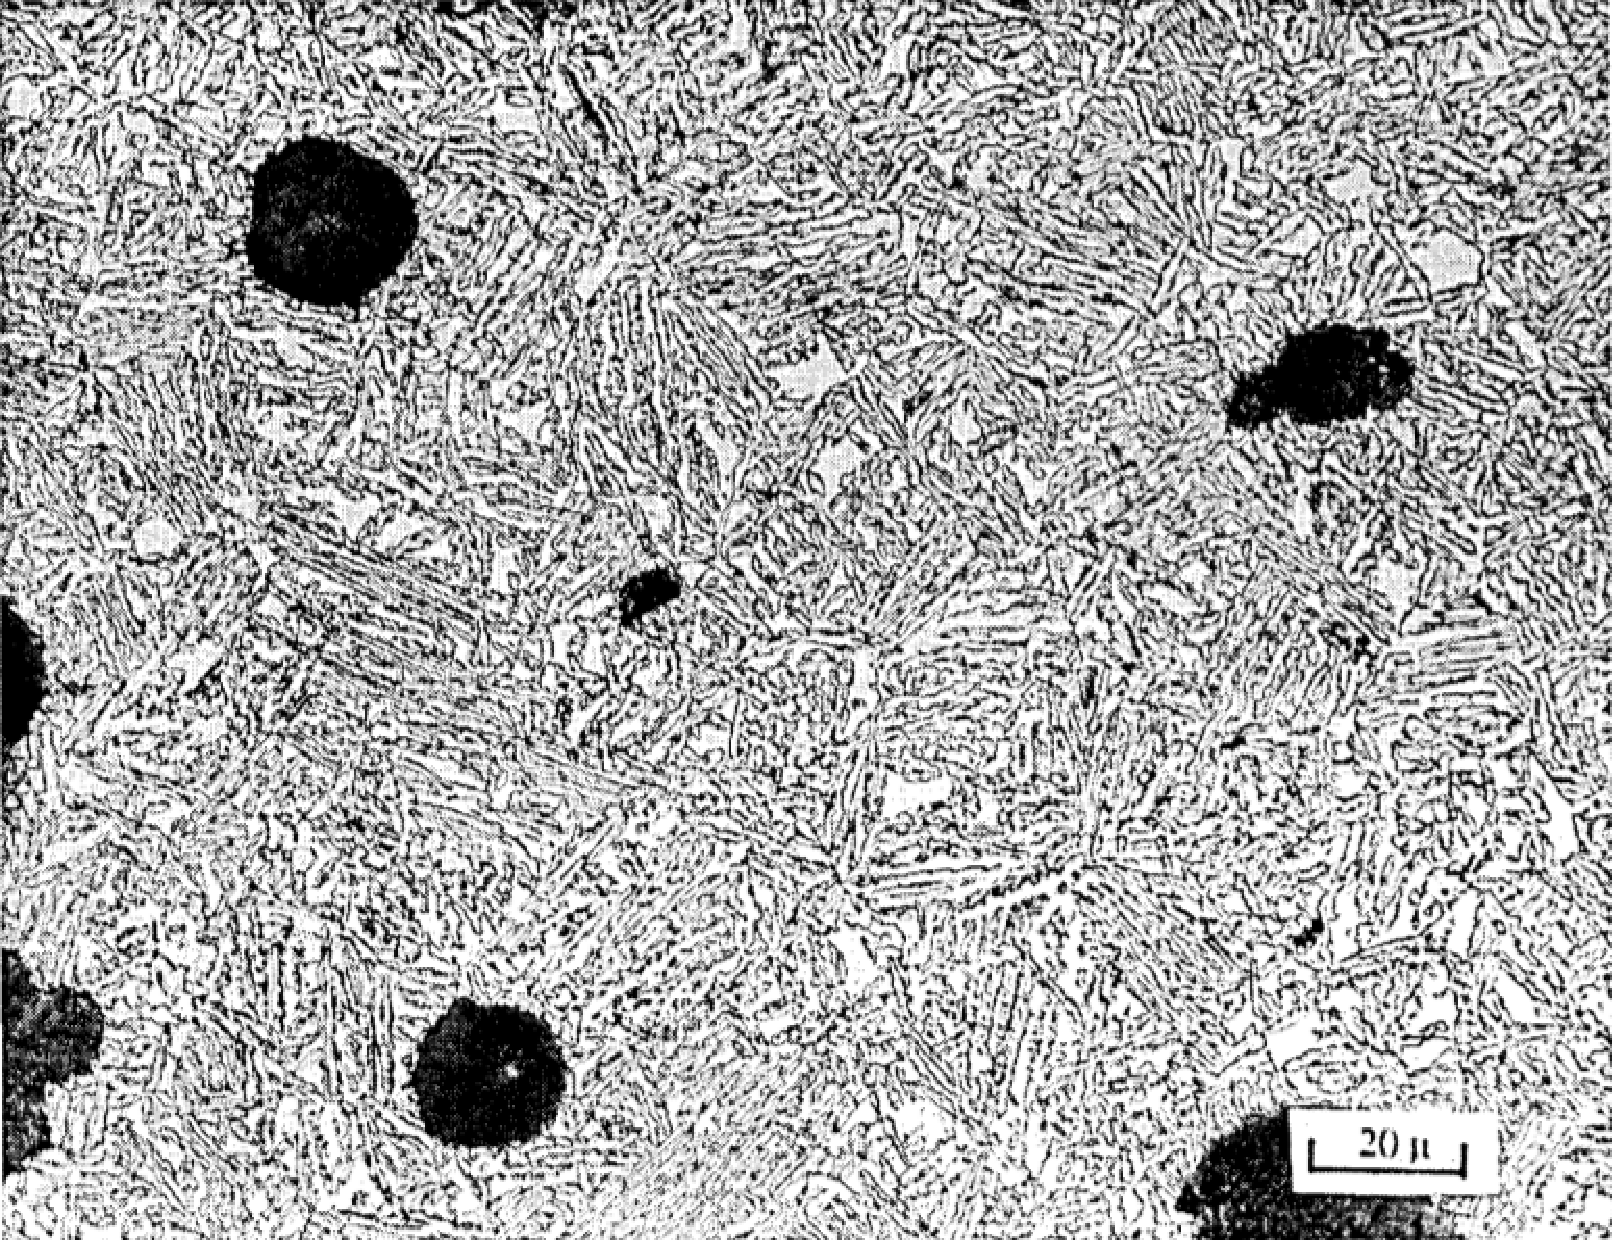
\includegraphics[height=5.8cm]{img/ADI360oC.pdf}}
	\quad
	\subfloat[]{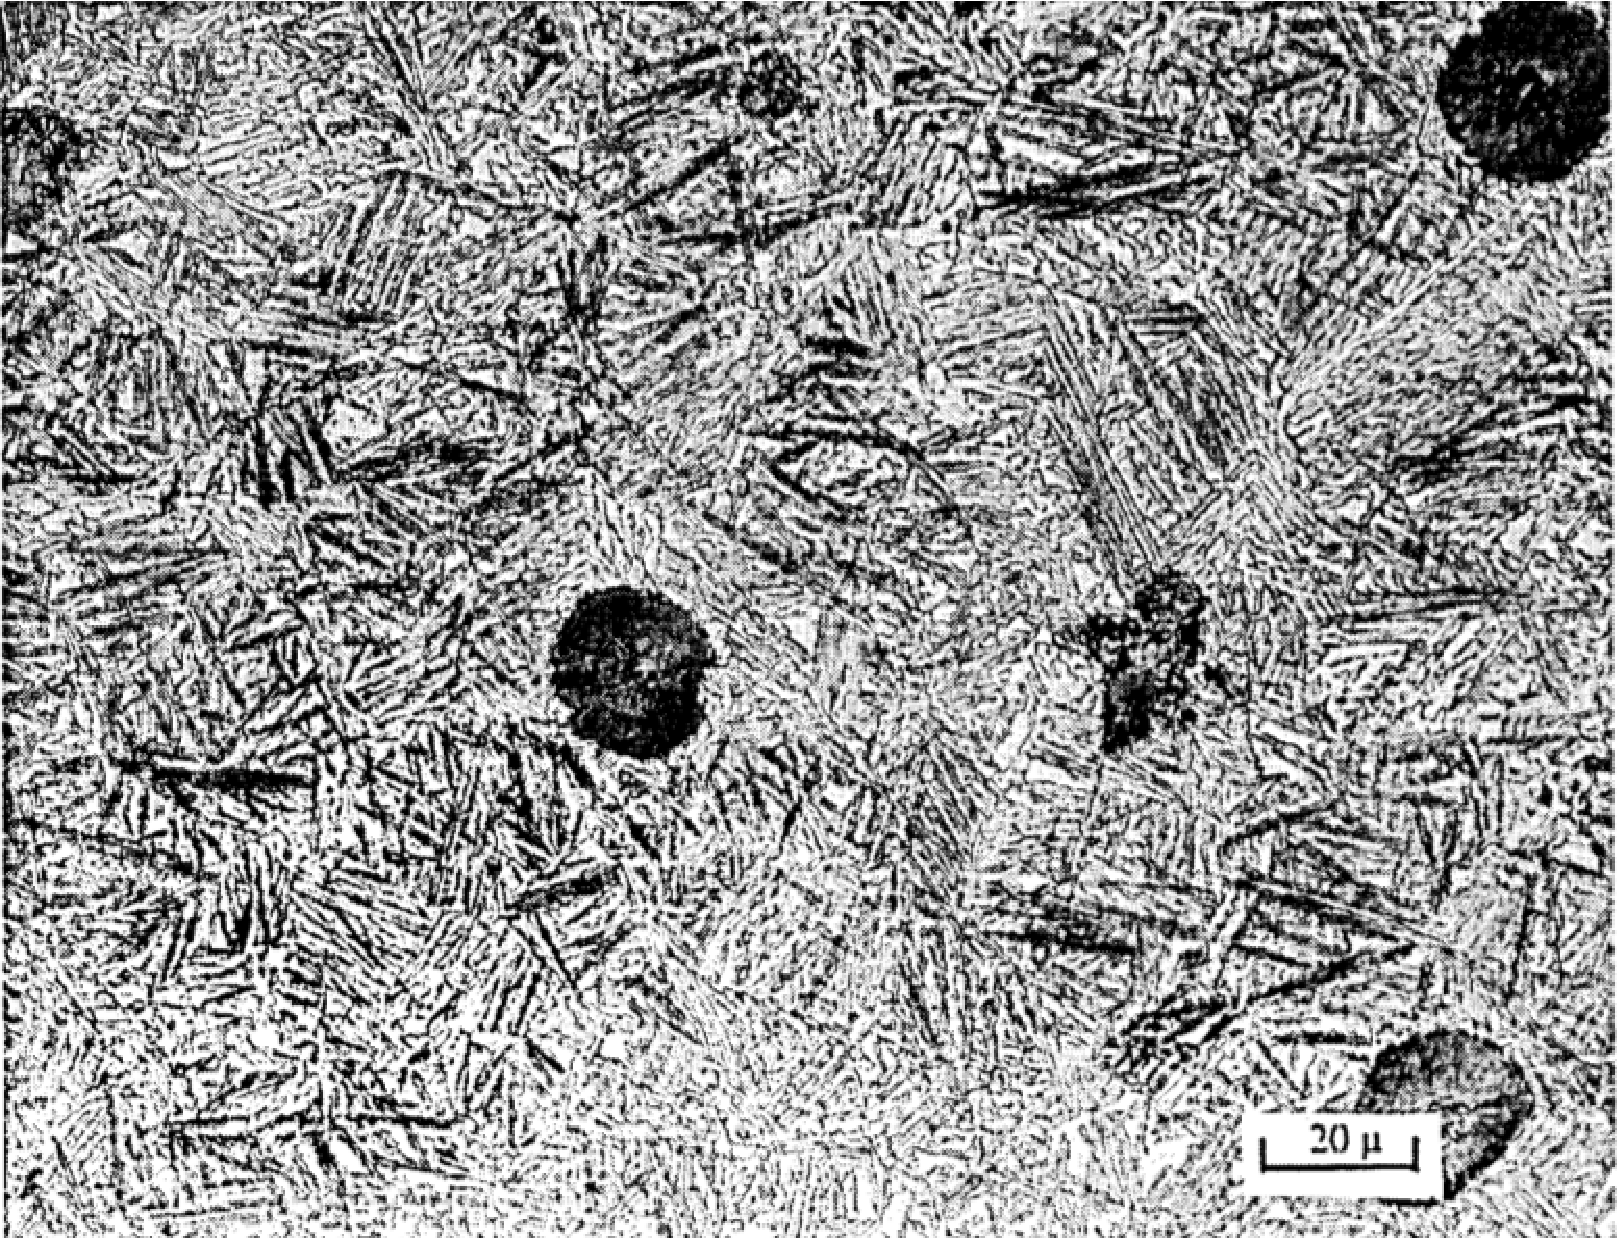
\includegraphics[height=5.8cm]{img/ADI310oC.pdf}}
	\caption{Microestruturas de ADIs produzidos pela austêmpera a (a) 360 °C e (b) 310 °C por uma hora. Imagens reproduzidas de\cite{Trudel1997}.}
	\label{fig:ADIs}
\end{figure}

Um aspecto importante da produção do ADI é o efeito da microsegregação na transformação bainítica no material. Como mencionado anteriormente, alguns autores reportam que é conveniente eliminar a microsegregação durante a etapa de austenitização. A justificativa para aplicação de tal medida é ilustrada na figura \ref{fig:cineticaADI}, que mostra esquematicamente o crescimento das colônias de ausferrita no ferro fundido. Devido à segregação nos contornos de células eutéticas, estas regiões possuem maior temperabilidade e, consequentemente, apresentam uma cinética mais lenta de transformação. \citaremsentenca{Trudel1997} reportam que estas regiões, por não se transformarem, devem estar empobrecidas em carbono e, dessa forma, embora já estejam enriquecidas por elementos que auxiliam na retenção da austenita, podem não reter totalmente a austenita na temperatura ambiente, se transformado parcialmente em martensita. \citaremsentenca{Bayati1995} mostraram que em um ferro nodular contendo 0,67\% de manganês, devido à diferença entre as cinéticas de transformação nas duas regiões, ocorre a superposição das etapas de transformação da ausferrita. Isto é, enquanto as regiões intercelulares ainda estão enriquecendo a austenita em carbono no primeiro estágio da reação, nas primeiras regiões a se transformar a precipitação de carbonetos já se iniciara. Este fenômeno leva à diminuição da janela de processo do material. \citaremsentenca{Meier2013a} fizeram observações semelhantes por meio de difração de nêutrons \enfase{in situ} e mostraram que a formação da ausferrita é associada a uma assimetria dos picos de difração da austenita, atribuída a fases com cinéticas de transformação diferentes.

\begin{figure}
	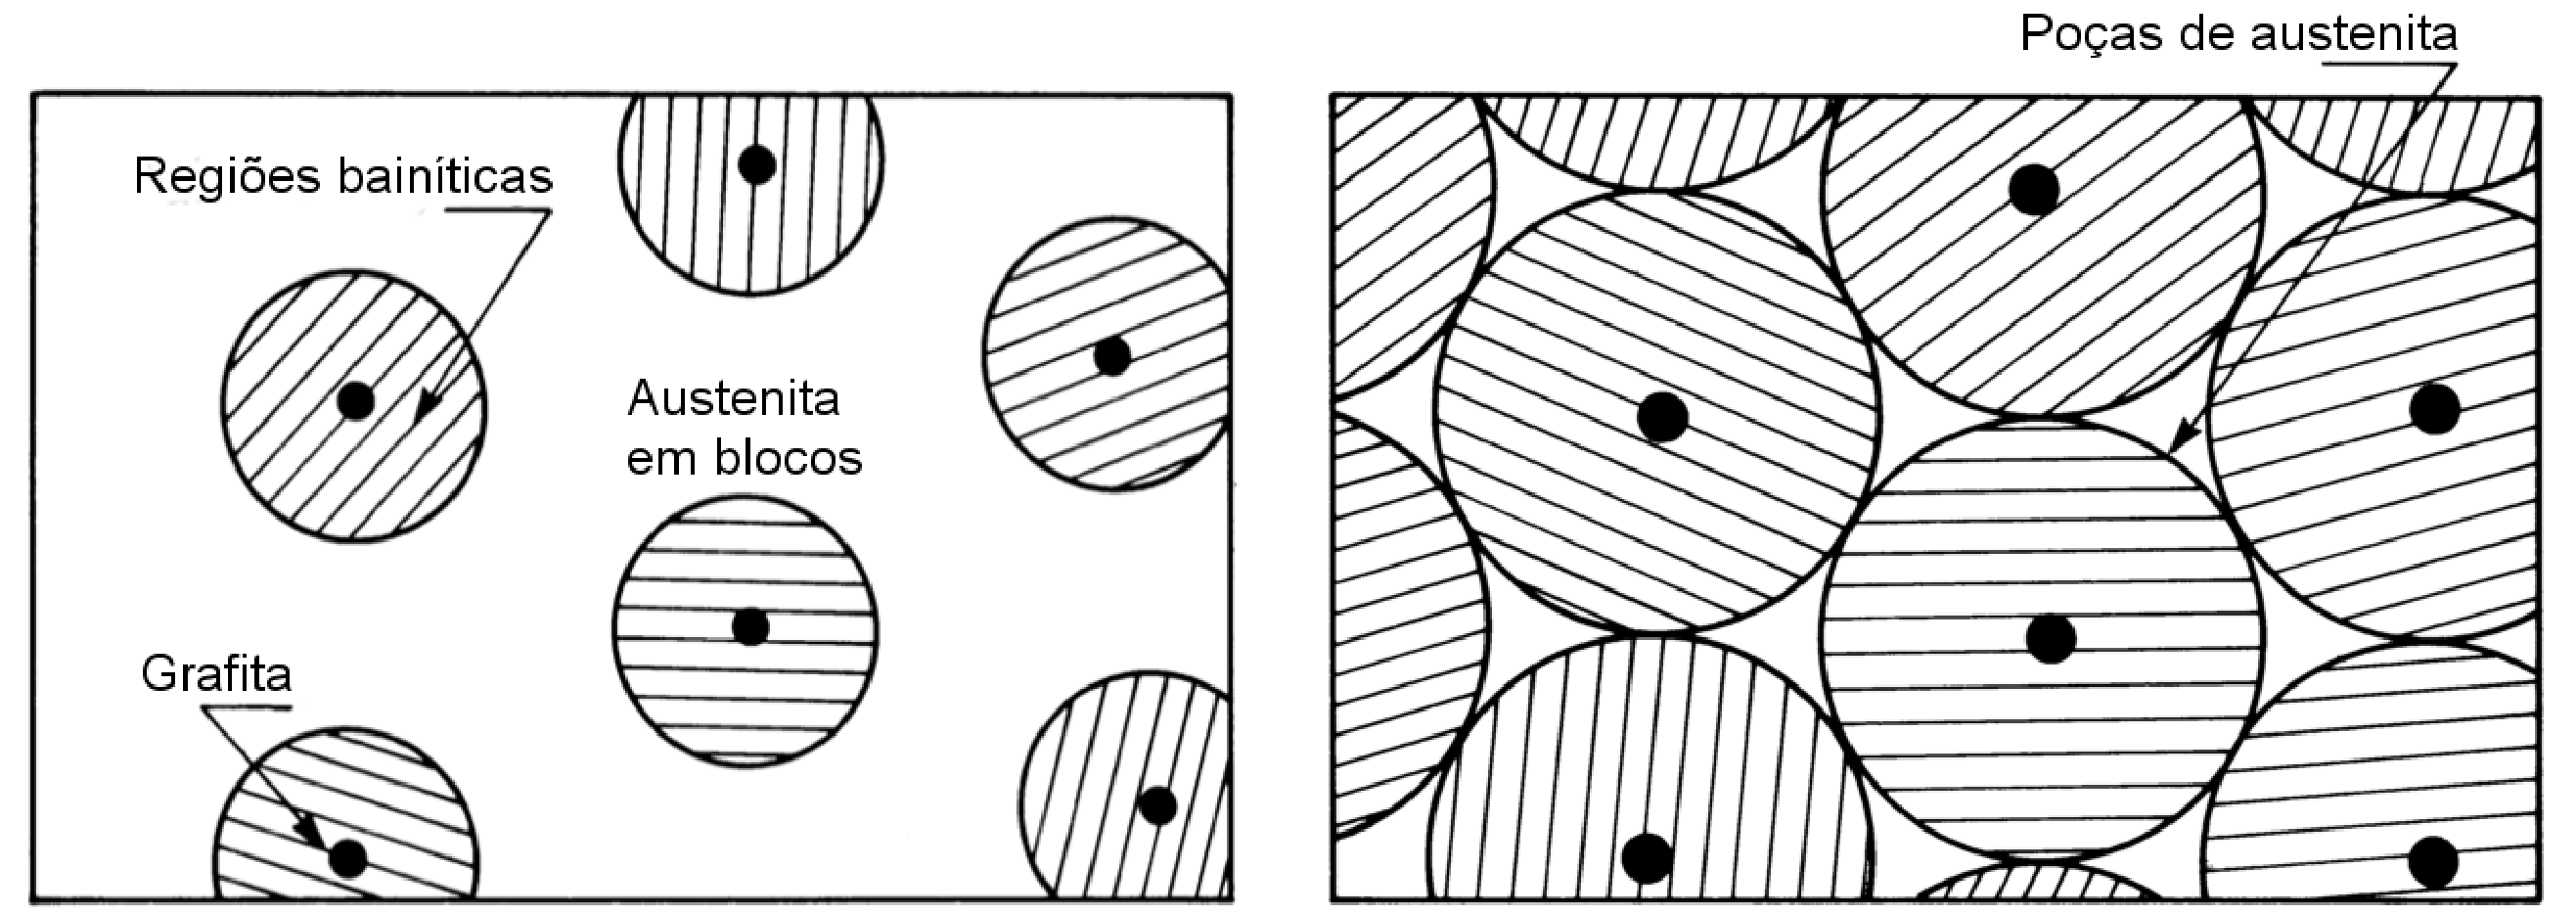
\includegraphics[width=16cm]{img/crescimentoAusferrita.pdf}
	\caption{Esquema representando, de forma simplificada, a evolução da formação de ausferrita em um ADI. A região hachurada corresponde à estrutura de ferrita bainítica entremeada por filmes de austenita enriquecida em carbono. As últimas poças não-trasformadas de austenita geralmente correspondem a contornos de célula eutética. Extraído de\cite{Aranzabal1997}.}
	\label{fig:cineticaADI}
\end{figure}


\section{Considera\c{c}\~{o}es sobre transforma\c{c}\~{o}es difusionais em ligas multicomponentes}

\label{sec:consTransf}

O atual desenvolvimento das teorias cinéticas de crescimento difusional de fases é em grande parte creditado ao trabalho pioneiro de \citaremsentenca{Zener1946}. Zener construiu um modelo cinético para o crescimento da ferrita a partir da austenita no sistema Fe-C. Para tanto, supôs que as composições na interface entre matriz e precipitado seriam dadas pelas linhas de solubilidade do diagrama de equilíbrio do sistema. Um tratamento mais completo necessita levar em conta vários elementos de liga, o que implica em um grande aumento de complexidade do problema no ponto de vista de modelamento do fenômeno. Particularmente, quando há a adição de elementos substitucionais, a diferença de mobilidade entre os solutos intersticial e substitucionais acarreta em situações de controle cinético com diferentes características, dependendo das forças motrizes às quais o material está sendo submetido. Assim, dependendo da velocidade da movimentação da interface, convém-se classificar as condições interfaciais em dois diferentes modos: equilíbrio local e paraequilíbrio.

\subsection{Equilíbrio local (EL)}
	
\novasigla{EL}{Equilíbrio local}

A condição de equilíbrio local é caracterizada pela movimentação lenta da interface, de modo a permitir que o equilíbrio local na interface entre precipitado e matriz seja estabelecido. Trata-se da situação assumida por Zener, em a igualdade dos potenciais químicos dos elementos na interface entre as duas fases é obedecida. A condição termodinâmica de EL no crescimento de ferrita ($\alpha$) a partir da austenita ($\gamma$) é dada por:

\begin{equation}
	\mu_i^\alpha = \mu_i^\gamma
\end{equation}
%
em que $\mu_i$ é o potencial químico do elemento $i$ (= C, Mn, Si, Cr, etc) na fase.

No que lhe diz respeito, ainda é possível discernir duas situações de EL, dependendo de como os solutos substitucionais são redistribuídos entre a fase em crescimento e a fase matriz.

Sob baixos super-resfriamentos, ocorre considerável redistribuição dos elementos substitucionais entre as duas fases. Nesta situação, conhecida como equilíbrio local com partição de soluto (EL-P)\novasigla{EL-P}{Equilíbrio local com partição de soluto}, a difusão dos substitucionais, por ser mais lenta do que a difusão dos elementos intersticiais, controla a movimentação da interface. Os perfis de composição na interface para a condição EL-P são mostrados na figura \ref{fig:modcineticos}a.

Sob forças motrizes maiores, a redistribuição do soluto substitucional entre as duas fases é mínima. Neste cenário, chamado de equilíbrio local com partição desprezível de soluto\novasigla{EL-PD}{Equilíbrio local com partição desprezível de soluto}, a composição das fases fora das redondezas da interface é praticamente a mesma. Por sua vez, nas proximidades da interface há a formação de uma ``crista'' (\enfase{spike}) de concentração de soluto (vide figura \ref{fig:modcineticos}b), de modo que as condições de equilíbrio sejam estabelecidas na interface e, portanto, a difusão do elemento intersticial controla a cinética da reação. Nesta condição, portanto, a movimentação da interface tende a ser mais rápida do que na situação de EL-P. %Não esquecer de pegar e citar artigos de Popov e Mikhalev, Darken, Kirkaldy e Hillert.\cite{Darken1961}\cite{Hillert1968}

\begin{figure}
	\subfloat[]{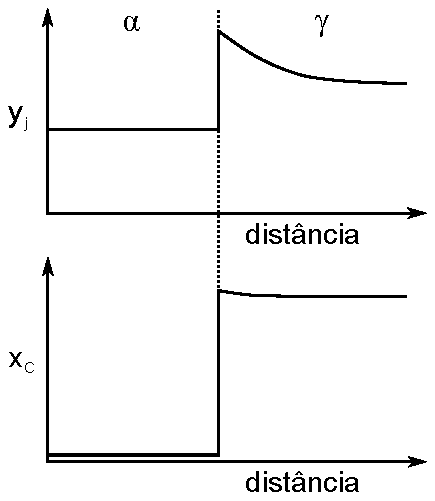
\includegraphics[height=5.8cm]{img/EL-P.pdf}}
	\hspace{1.5cm}
	\subfloat[]{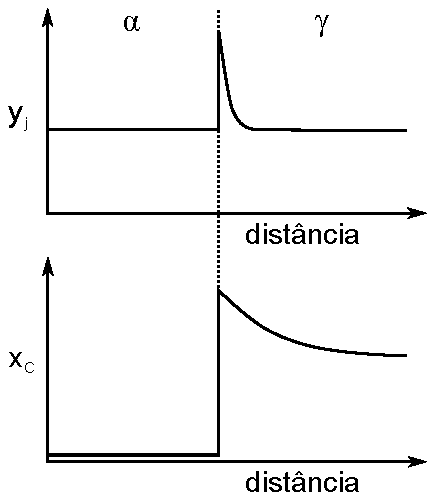
\includegraphics[height=5.8cm]{img/EL-PD.pdf}}
	\vspace{0pt}
	\subfloat[]{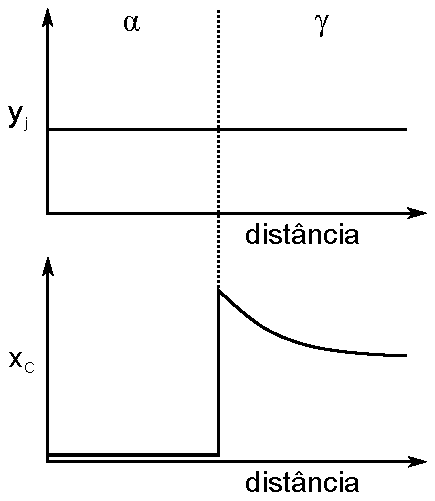
\includegraphics[height=5.8cm]{img/PE.pdf}}
	\caption{Perfis de composição ($x_C$) e fração de sítios substitucionais ($y_j$) na ferrita ($\alpha$) e na austenita ($\gamma$) segundo os modelos cinéticos de (a) equilíbrio local com partição de soluto (EL-P); (b) equilíbrio local com partição desprezível de soluto (EL-PD); e (c) paraequilíbrio (PE).}
	\label{fig:modcineticos}
\end{figure}

\subsection{Paraequilíbrio (PE)}

\novasigla{PE}{Paraequilíbrio}

\citaremsentenca{Hultgren1947} observou que, durante a decomposição eutetóide da austenita em ferrita e cementita, o produto formado usualmente herdava a mesma composição de elementos substitucionais da fase matriz. Ele chamou estes produtos de paraferrita e paracementita, em oposição às fases de equilíbrio pleno. Em adição, Hultgren argumentou que o crescimento destas \enfase{parafases} ocorreria segundo uma condição termodinâmica específica, denominada paraequilíbrio, na qual duas fases estariam em equilíbrio real uma em relação à outra apenas com respeito aos componentes de maior mobilidade, ou seja, os elementos intersticiais.

A situação de paraequilíbrio ocorre devido à grande diferença de mobilidade entre os solutos substitucionais e o soluto intersticial. Esta situação é passível de ocorrer em baixas temperaturas, quando a difusão dos substitucionais é lenta\cite{Hillert1953}. Adicionalmente, se os elementos substitucionais são impedidos de se redistribuir, seus potenciais químicos individuais não podem ser igualados. Dessa maneira, o comportamento termodinâmico do sistema deve ser avaliado pelo potencial químico $\mu_Z$ do elemento hipotético $Z$\cite{Ghosh2001}, de modo a serem obedecidas as relações termodinâmicas que regem o paraequilíbrio:

\begin{subequations}
	\begin{align}
		\mu_C^\alpha &= \mu_C^\gamma \label{eq:potQuimC}\\
		y_j^\alpha &= y_j^\gamma \label{eq:fracSitios}\\
		\mu_Z^\alpha \left ( \equiv \sum y_j^\alpha \mu_j^\alpha \right) &= \mu_Z^\gamma \left ( \equiv \sum y_j^\gamma \mu_j^\gamma \right ) \label{eq:potQuimZ}
	\end{align}
\end{subequations}
%
em que $y_j$ são as frações de sítios substitucionais do elemento $j$ (= Mn, Si, Cr, Ni, etc.) nas fases matriz $\gamma$ e em crescimento $\alpha$. Note-se que o potencial químico do elemento teórico $Z$ é definido como a soma dos potenciais químicos dos elementos substitucionais ponderados pelas suas respectivas frações de sítios na fase. Por sua vez, para um sistema que contém tanto elementos substitucionais, quanto um elemento intersticial (no caso, o carbono), $y_j$ se correlaciona com a fração molar $x_j$ do substitucional na fase pela expressão:

\begin{equation}
	y_j = \frac{x_j}{1 - x_C}
\end{equation}
%
em que $x_C$ é a fração molar do carbono na fase.

A figura \ref{fig:modcineticos}c ilustra esquematicamente os perfis de composição no crescimento da ferrita a partir da austenita obedecendo as condições de paraequilíbrio. É importante ressaltar que, segundo a definição de Hultgren, tanto as fases formadas segundo o mecanismo de paraquilíbrio, quanto pelo mecanismo de equilíbrio local com partição desprezível de soluto são consideradas parafases. Na situação de EL-PD, embora as composições na interface obedeçam o equilíbrio pleno local, os teores médios de substitucionais em cada fase são praticamente os mesmos\cite{Hillert2004a}.


\section{Transforma\c{c}\~{a}o Martens\'{i}tica}

\label{sec:Martensita}

Nas ligas ferrosas contendo carbono, quando a decomposição eutetóide da austenita, controlada pela difusão dos elementos de liga, é evitada pelo rápido resfriamento do material a partir da temperatura de autenitização, a austenita tende a se decompor por um mecanismo não difusional na fase metáestável martensita. Nestas ligas a transformação martensítica normalmente gera uma fase de estrutura cristalina tetragonal de corpo centrado em temperaturas inferiores à temperatura de início da transformação martensítica (temperatura Ms). Em situações especiais é possível que uma martensita de estrutura hexagonal compacta se forme a partir da austenita. Outros sistemas de ligas também apresentam transformação do tipo martensítica, mas a importância tecnológica da martensita de ligas baseadas no elemento ferro supera todas as aplicações dos demais sistemas.

\simbolo{Ms}{Temperatura de início da transformação martensítica}

A transformação martensítica em aços carbono é acompanhada de expansão volumétrica do material, tal qual ocorre na formação da ferrita a partir da austenita. Como não há redistribuição de soluto entre as duas fases, o produto resultante herda a composição química da fase ancestral de austenita. A presença dos elementos químicos em solução sólida na martensita, em especial o carbono, desempenha papel crítico em seu endurecimento. A formação da martensita é acompanhada da ocupação de posições assimétricas nos sítios intersticiais octaédricos pelos átomos de carbono, fenômeno que leva ao estabelecimento da tetragonalidade da martensita\cite{Zener1946,Hillert1986}. Adicionalmente, a cristalografia da transformação martensítica requer que uma deformação cisalhante seja aplicada à célula unitária da austenita, como teorizado por Bain\cite{Bain1924}. Para compensar este cisalhamento, de modo que um plano invariante macroscópico seja mantido entre as duas fases, é necessário que a martensita recém formada sofra uma distorção para ser acomodada na austenita. Essa distorção é conhecida como deformação de plano invariante\cite{Honeycombe2006} e em magnitude é tão maior quando maior a tetragonalidade da martensita. Como ilustrado na figura \ref{fig:cisMartensita}, essa deformação pode ser obtida por meio do escorregamento de planos cristalinos e consequente criação de discordâncias no interior da fase, ou pela criação de defeitos de maclas na martensita.

\begin{figure}
	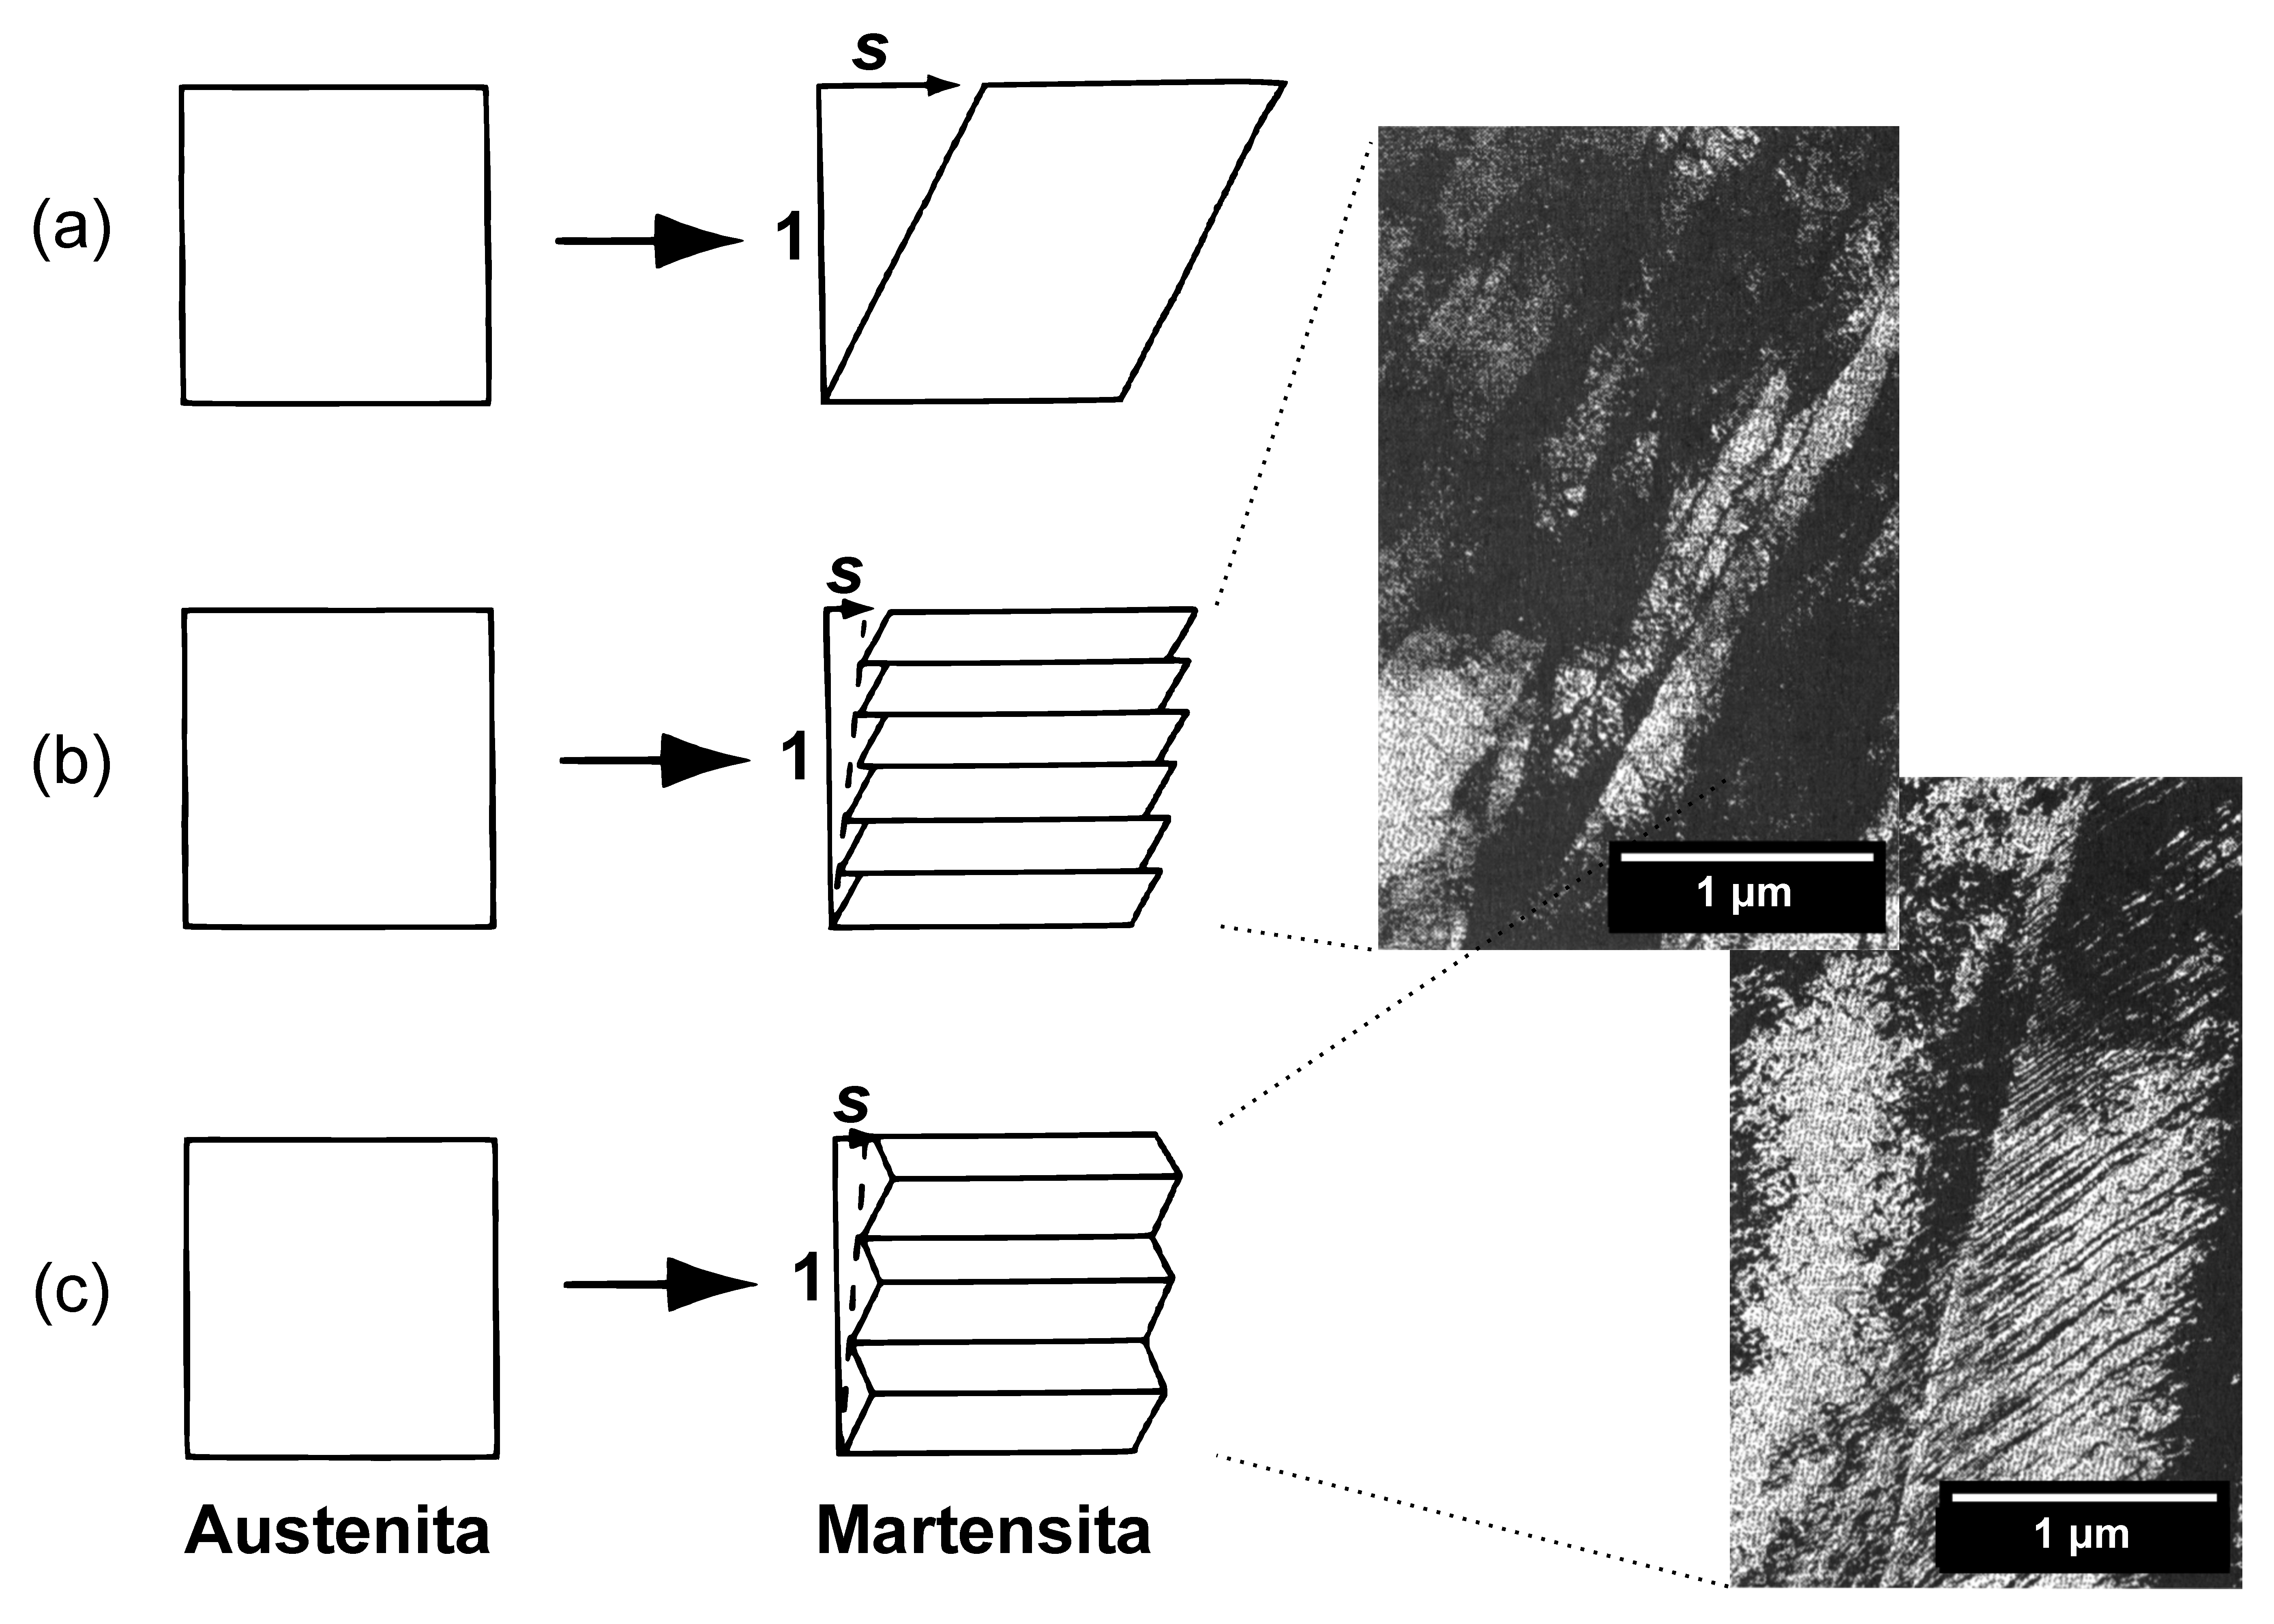
\includegraphics[width=14cm]{img/shearMartensite.pdf}
	\caption{Figura ilustrando que tanto (b) escorregamento quanto (c) maclação podem compensar o cisalhamento \textit{s} produzido pela deformação de Bain esquematizada em (a). No detalhe, imagens obtidas por microscopia eletrônica de transmissão das microestruturas dos dois tipos de martensita. Adaptado de\cite{Porter2009}.}
	\label{fig:cisMartensita}
\end{figure}

A tetragonalidade da martensita aumenta com fração de sítios intersticiais ocupados por átomos de carbono. Consequentemente, os defeitos cristalinos relacionados à deformação de plano invariante são mais extensos em ligas de alto carbono. Esse raciocínio leva à conclusão de que a martensita de médio e alto carbono possui elevada dureza, associada, porém, a valores muito baixos de alongamento. Por outro lado, a martensita formada em ligas de baixo carbono pode apresentar estrutura cristalina cúbica de corpo centrado após um certo período de envelhecimento. \citaremsentenca{Speich1972} pontuaram que este fenômeno se deve à segregação do carbono para discordâncias e contornos de ripas de martensita, sendo que o ponto de saturação dos defeitos cristalino ocorre em torno de 0,2\%C.

A natureza da deformação de plano invariante é utilizada para classificação da morfologia da martensita. Assim, a martensita acomodada pela formação de discordâncias e acionamento de planos de escorregamento é denominada martensita escorregada ou, em virtude de sua morfologia característica, martensita em ripas. Por sua vez, a martensita constituída de maclas é chamada de martensita maclada ou em placas. A predominância da ocorrência de uma morfologia ou outra está normalmente associada à composição química da austenita antecessora. Como mostra a figura \ref{fig:MsZhaoNotis}, dada uma composição fixa, a cada morfologia de martensita é associada uma temperatura Ms. O aumento do teor de carbono leva à diminuição simultânea das duas temperaturas Ms, mas esta tendência é maior para a martensita em ripas. Assim, teores de carbono mais elevados favorecem a formação de martensita em placas, enquanto para aços pouco ligados a martensita em ripas predomina. Por sua vez, a têmpera em aços com teores de carbono intermediários gera microestruturas mistas.

\begin{figure}
	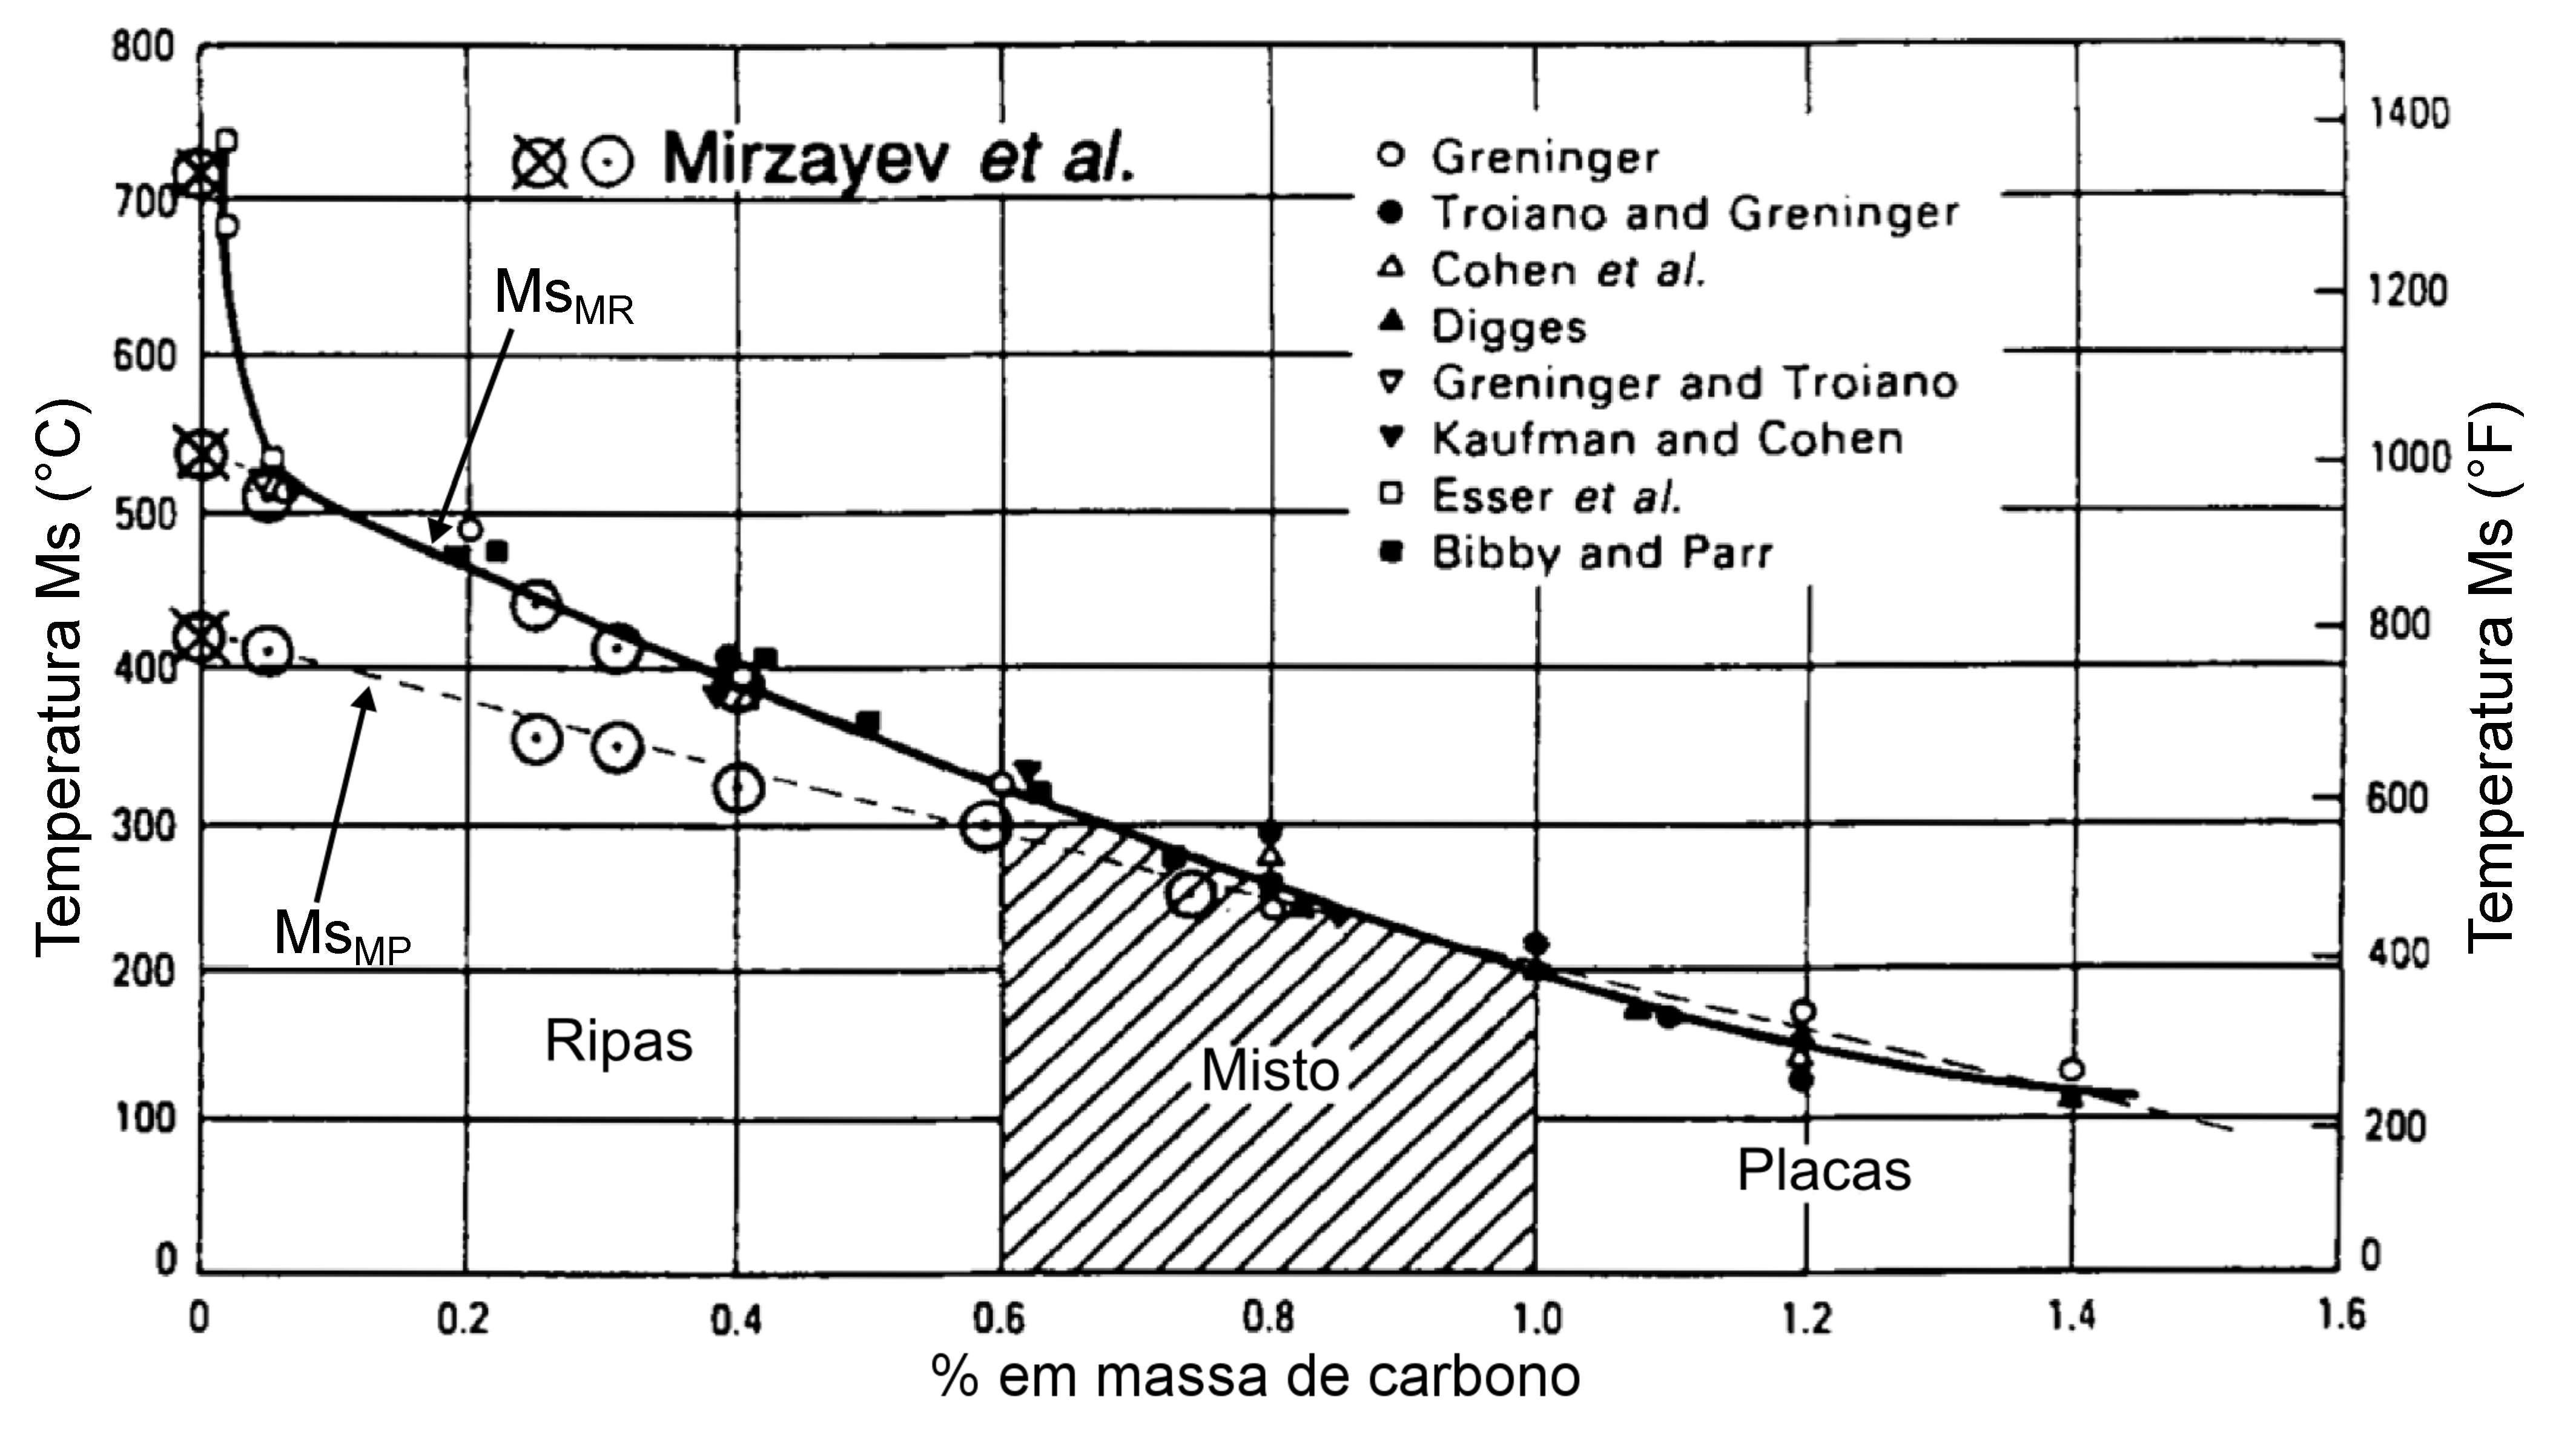
\includegraphics[width=16cm]{img/Ms_Zhao.pdf}
	\caption{Variação das temperaturas início de formação da martensita escorregada ou em ripas ($Ms_{MR}$) e martensita maclada ou em placas ($Ms_{MP}$) em função da composição de ligas Fe-C. Adaptado de\cite{Zhao1995}.}
	\label{fig:MsZhaoNotis}
\end{figure}

Outros elementos de liga também são conhecidos por desempenhar a diminuição da temperatura Ms. De fato, dentre os mais comuns elementos de liga empregados na elaboração de  aços e ferros fundidos, apenas o cobalto é conhecido por elevar a temperatura Ms\cite{Honeycombe2006}. Várias equações empíricas reportadas na literatura foram desenvolvidas para quantificar o efeito dos elementos de liga nesse parâmetro. A mais utilizada é provavelmente a equação de \citaremsentenca{Andrews1965}:

\begin{equation}
	Ms = 539 - 423\%w_C^\gamma - 30,4\%w_{Mn}^\gamma - 17,7\%w_{Ni}^\gamma - 12,1\%w_{Cr}^\gamma - 7,5\%w_{Mo}^\gamma
	\label{eq:Andrews}
\end{equation}
%
em que $\%w_i^\gamma$ é a porcentagem em massa do elemento $i$ (= C, Mn, Ni, Cr, Mo) dissolvido na austenita. É notável que o efeito do carbono é consideravelmente mais pronunciado do que o dos demais elementos químicos.

A equação de Andrews vale para uma faixa limitada de composições, em geral prevendo razoavelmente bem a temperatura Ms para baixos teores de elementos de liga. Para aços muito ligados, termos de ordem quadrática costumam a pesar na contabilização do efeito do elemento, distanciando a estimativa dos valores experimentais. Além disso, a equação não contabiliza o efeito de alguns importantes elementos de liga empregados na siderurgia moderna, como microligantes (e.g., Ti, Nb, V) e elementos utilizados para supressão da precipitação de carbonetos (Si e Al). Uma compilação das equações empíricas disponíveis na literatura para o cálculo do Ms é disponível no trabalho de \citaremsentenca{Liu2001}, sendo reforçado pelos autores que as equações são somente válidas para aços de baixa liga.

Outro aspecto importante do entendimento da transformação martensítica é a determinação da fração transformada em função da temperatura de reação. Como a transformação martensítica ocorre sem difusão, dada uma taxa de resfriamento fixa, a fração transformada de martensita deve depender apenas do super-resfriamento abaixo da temperatura Ms, e não do tempo de permanência na temperatura de têmpera $TT$, como expresso na equação empírica de \citaremsentenca{Koistinen1959}:

\begin{equation}
	f^\gamma = 1 - f^{\alpha\text{\textquoteright}} = \exp \left[ \beta \left ( Ms - TT \right )\right ]
	\label{eq:KM}
\end{equation}
%
em que $f^{\alpha\text{\textquoteright}}$ e $f^\gamma$ são, respectivamente, a fração transformada de martensita e a fração não-transformada de austenita, enquanto $\beta$ é um coeficiente de ajuste que em várias ligas assume o valor de $-1,1 \times 10^{-2} \text{°C}^{-1}$. Este parâmetro pode sofrer variações de acordo com a composição e parâmetros de tratamento térmico do material. $\beta$ pode ser determinado sob cada condição por meio de medidas experimentais globais, tais quais as realizadas em experimentos de dilatometria e resistividade elétrica\cite{DeMoor2009}.

Um fato previsto pela equação de Koistinen-Marburger é que ligas com baixas temperaturas Ms devem reter grandes quantidades de austenita não-transformada na temperatura ambiente. Assim, tendo em vista a interpretação da equação de Andrews (equação \ref{eq:Andrews}), salvo o caso citado do elemento cobalto, quanto maior o teor de elementos de liga na austenita, maior sua capacidade de ser retida na temperatura ambiente.

É importante ser ressaltado, porém, que a generalização sobre a atuação dos elementos de liga no controle da proporção das fases após a têmpera só é possível porque a mistura martensita + austenita está distante do equilíbrio termodinâmico.\citaremsentenca{Honeycombe2006} classificam elementos de liga nos aços em duas categorias: alfagênicos e gamagênicos, ou seja, estabilizadores da ferrita (fase $\alpha$) ou da austenita (fase $\gamma$). Nesta distinção, os elementos são classificados de acordo com sua capacidade de ampliar ou contrair o campo austenítico do ferro em temperaturas elevadas, segundo o diagrama de equilíbrio. Esse argumento leva, por exemplo, a afirmações aparentemente contraditórias, mas verídicas, como o fato do elemento cromo contrair o campo austenítico, mas, quando em solução sólida na austenita, favorecer sua retenção após a têmpera do material.

Neste texto, o conceito de estabilidade da austenita foi adotado em um sentido menos rigoroso, denotando a capacidade da fase manter suas propriedades após sua exposição a solicitação mecânica e condições cinéticas (tempo e temperatura) favoráveis para sua decomposição.

%efeito TRIP é abordado na seção \ref{subsec:TRIP}. Transfomação isotérmica da martensita são abordados na seção \ref{subsec:decompMs}

\subsection{Estabilidade mec\^{a}nica da austenita e efeito TRIP}

\label{subsec:TRIP}

Ainda que a austenita seja retida à temperatura ambiente, em decorrência de sua metaestabilidade termodinâmica, caso seja fornecida alguma espécie de ativação ao material, esta fase pode se decompor em produtos que reduzem a energia livre do sistema. O efeito TRIP (\enfase{Transformation-induced plasticity}) acontece quando a austenita é submetida a um trabalho de deformação plástica e se transforma em martensita. A transformação martensítica induzida por tensões locais tem o efeito de aliviar a concentração de tensões, aumentando a taxa de encruamento e promovendo deformação homogênea, com consequentes melhorias na resistência, ductilidade e tenacidade do material\cite{Honeycombe2006}.

Em aços inoxidáveis austeníticos este fenômeno é bem conhecido. %pegar ou o trabalho do Wasserman, ou o trabalho do Zackay. vide \cite{DeCooman2004}
Nestas ligas, a deformação plástica leva primeiramente à formação de martensita hexagonal nucleada nas falhas de defeito de empilhamento (maclas), sendo subsequentemente transformada em martensita tetragonal\cite{Honeycombe2006}. O efeito TRIP, no entanto, só ocorre quando a deformação é aplicada em temperaturas abaixo de uma temperatura $Md$ característica da fase. Quanto maior a temperatura, maior a energia de defeito de empilhamento (EDE) da austenita e, portanto, maior a força motriz para que a transformação ocorra. Logo, a temperatura $Md$ define termodinamicamente o ponto em que o trabalho de deformação aplicado ao material é compensado pela EDE\cite{DeCooman2004}.

A estabilidade mecânica da austenita, no entanto, define se o fenômeno TRIP trará os benefícios enumerados acima ao material. Não é desejável que a temperatura $Md$ seja maior do que a temperatura de utilização do material, de modo que o fenômeno TRIP não ocorra. Por outro lado, caso a austenita se deforme sob aplicação de tensões/deformações muito pequenas, o material também não terá melhoria em ductilidade. Reporta-se na literatura que há uma quantidade ótima de carbono na austenita retida que aumenta o alongamento; valores muito baixos ou muito altos não produzem melhoria do alongamento\cite{Reisner1997,Meyer1999}.

Além disso, o condicionamento da microestrutura também afeta a estabilidade mecânica da austenita. Tamanho, morfologia e distribuição da austenita na microestrutura são variáveis que definem o comportamento mecânico desta fase\cite{Timokhina2004}. Grãos menores de austenita contêm menos sítios potenciais para nucleação de martensita. Assim, regiões que contêm grãos grosseiros e/ou blocos isolados de austenita tendem a ser mais instáveis e transformam-se facilmente, contribuindo pouco para o aumento da ductilidade. Por outro lado, grãos submicrométricos de austenita possuem menor tendência de se transformar e a austenita acaba sofrendo intenso encruamento, contribuindo pouco com o efeito TRIP\cite{Bai1998}. Por sua vez, materiais que apresentam austenita na forma de filmes entre subunidades de bainita isenta de carbonetos e entre ripas de martensita apresentam melhor comportamento em relação ao alongamento\cite{Takahashi1991,Xiong2013}.

Ligas modernas são produzidas com quantidades controladas de austenita estabilizada para se beneficiar do efeito TRIP. Um exemplo destes aços multifásicos que já tem atingido alto volume de aplicações são chapas de aços TRIP (\enfase{TRIP-assisted steels}) para aplicações na indústria automotiva. Estes aços contém uma estrutura de ferrita equiaxial produzida pela austenitização parcial no campo intercrítico e bainita isenta de carbonetos entremeada com austenita retida, produzida por um tratamento de austêmpera. Assim como nos ADIs, o projeto de liga destes aços contém teores controlados de silício, alumínio ou fósforo para evitar a precipitação de carbonetos durante a reação bainítica, permitindo a partição de carbono para estabilizar a austenita não transformada \cite{DeCooman2004,Honeycombe2006}.

O processo de Têmpera e Partição também tem como objetivo a produção de microestruturas multifásicas contendo austenita retida estabilizada à temperatura ambiente. Este tópico é abordado na próxima seção do texto.

\section{O processo de T\^{e}mpera e Parti\c{c}\~{a}o (T\&P)}

\label{sec:processoTP}
 
O caráter frágil da martensita virgem exige que tratamentos térmicos subsequentes sejam aplicados ao material para que exigências de tenacidade sejam obedecidas. O tratamento de revenimento consiste do tratamento isotérmico da martensita em temperaturas na faixa de 150 a 700 °C. O propósito do revenimento é fornecer ativação térmica ao material para que a microestrutura se aproxime do estado de equilíbrio\cite{Honeycombe2006}. Assim, as reações do revenimento promovem a decomposição da austenita não-transformada (retida) e o alívio da supersaturação de carbono da martensita para formação de microestruturas que minimizam a energia livre do sistema.

A redistribuição do carbono da martensita para a austenita durante o revenimento é um fato conhecido a longa data\cite{Matas1960}. No entanto, sobretudo devido à formação de carbonetos desde as etapas iniciais do revenimento, até recentemente este fato nunca fora aproveitado para o desenvolvimento de microestruturas de interesse tecnológico. Em 2003, \citaremsentenca{Speer2003} afirmaram que quando a precipitação de carbonetos é suprimida, a \enfase{partição} do carbono da martensita para austenita poderia ser conseguida mesmo em altas temperaturas. Nesse trabalho, os autores apresentaram um modelo termodinâmico para determinar o teor de carbono na austenita após a partição de carbono e predição da microestrutura de uma nova rota de tratamento térmico denominada \sigla{T\&P}{Têmpera e Partição} baseada nos conceitos de controle da fração transformada de martensita e de estabilização da austenita pelo seu enriquecimento de carbono.

O processo T\&P é esquematizado na figura \ref{fig:esqTP}. Após a austenitização total ou parcial da liga, o material é temperado até uma temperatura TT abaixo da temperatura Ms para produzir uma mistura controlada de martensita e austenita. Na sequência, na etapa de partição, o material é mantido em um patamar isotérmico em uma temperatura TT (T\&P em uma etapa) ou em uma temperatura de partição TP mais elevada (T\&P em duas etapas) para permitir a partição de carbono da martensita para a austenita. Como discutido anteriormente, o carbono em solução sólida diminui a temperatura Ms da austenita, eventualmente para temperaturas inferiores à ambiente e, nesse caso, mantém-na estabilizada à temperatura ambiente. A viabilidade do processo T\&P depende da supressão da precipitação de carbonetos durante a etapa de partição, que consumiriam parcela do carbono da austenita. Para tanto, são empregados elementos de liga que retardam essas reações, como os já citados silício, alumínio e fósforo.

\begin{figure}
	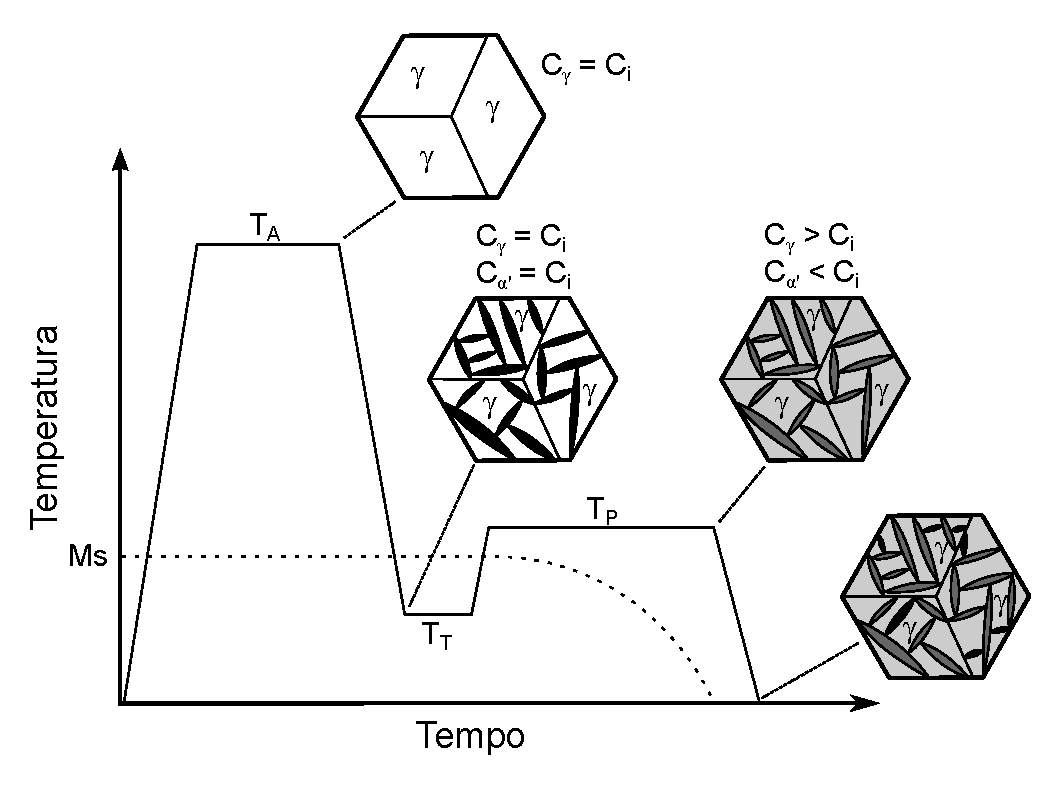
\includegraphics[height=9cm]{img/esquemaTP.pdf}
	\caption{Figura esquemática do tratamento de Têmpera e Partição (T\&P). TA, TT e TP representam as temperaturas de austenitização, de têmpera e do tratamento de partição, enquanto $C_{i}$, $C_{\gamma}$ e $C_{\alpha\text{'}}$ representam as concentrações de carbono inicial, da austentita e da martensita, respectivamente. Adaptado da referência\cite{Edmonds2006}. }
	\label{fig:esqTP}
\end{figure}

Uma vez que permite controlar de uma forma relativamente fácil a microestrutura do material, o processo T\&P é capaz de produzir a partir de uma mesma formulação de liga, materiais com diferentes comportamentos mecânicos. A martensita particionada confere resistência mecânica semelhante à obtida durante o tratamento de revenimento, enquanto a austenita confere ductilidade e tenacidade em virtude da ocorrência do fenômeno TRIP\cite{Matlock2010}. Por estes motivos, materiais temperados e particionadas tem sido produzidos no desenvolvimento de chapas de aços de alta resistência, atingindo combinações de propriedades atribuídas a uma classe inteiramente nova de aços.

\citaremsentenca{Matlock2003c} conduziram investigação inicial do conceito T\&P em barras de aços médio carbono (0,35\% em massa) microligado. Os autores verificaram grande quantidade de austenita retida enriquecida em carbono no produto final, embora aparente formação de carbonetos de transição não fora evitada durante a etapa de partição. Gendermann apud\cite{Speer2004} examinou as propriedades mecânicas de aço AISI 9260 modificado com adição de teores elevados de Si (2\% em massa) submetido ao processo T\&P, avaliando as variáveis temperatura de têmpera e tempo e temperatura de partição. Quantidades de austenita próximas a 30\% em volume foram obtidos para amostras temperadas a 190 °C e particionadas a 500 °C por 10 segundos. Quantidades significativas de austenita retida não foram obtidas quando o material fora temperado e revenido, enquanto menores valores de dureza foram obtidos para o material austemperado.

Como mencionado na seção \ref{subsec:TRIP}, aços TRIP contém quantidades significativas de austenita estabilizada, esta produzida pela interrupção da reação bainítica durante a estase, e também fazem uso de elementos de liga para suprimir a precipitação de carbonetos. Dessa forma, é natural que ligas semelhantes às utilizadas nestes aços sejam submetidas ao processo de Têmpera e Partição. \citaremsentenca{Streicher2004} %Arranjar futuramente o documento desse artigo http://digital.library.aist.org/pages/PR-255-006.htm
avaliaram os aspectos de transformações de fases e a resposta a solicitações mecânicas de um aço ligado ao silício (1,63\% em massa) submetido ao processo T\&P. Variações do processamento envolveram a realização do tratamento térmico em uma ou duas etapas. As combinações de propriedades dos materiais temperados e particionados forneceram valores semelhantes de resistência à tração associados a valores de alongamento mais elevados do que a classe de aços martensíticos. Estes resultados, comparados a outras classes de aços modernos, são mostrados na figura \ref{fig:TRIPQP}.

\begin{figure}
	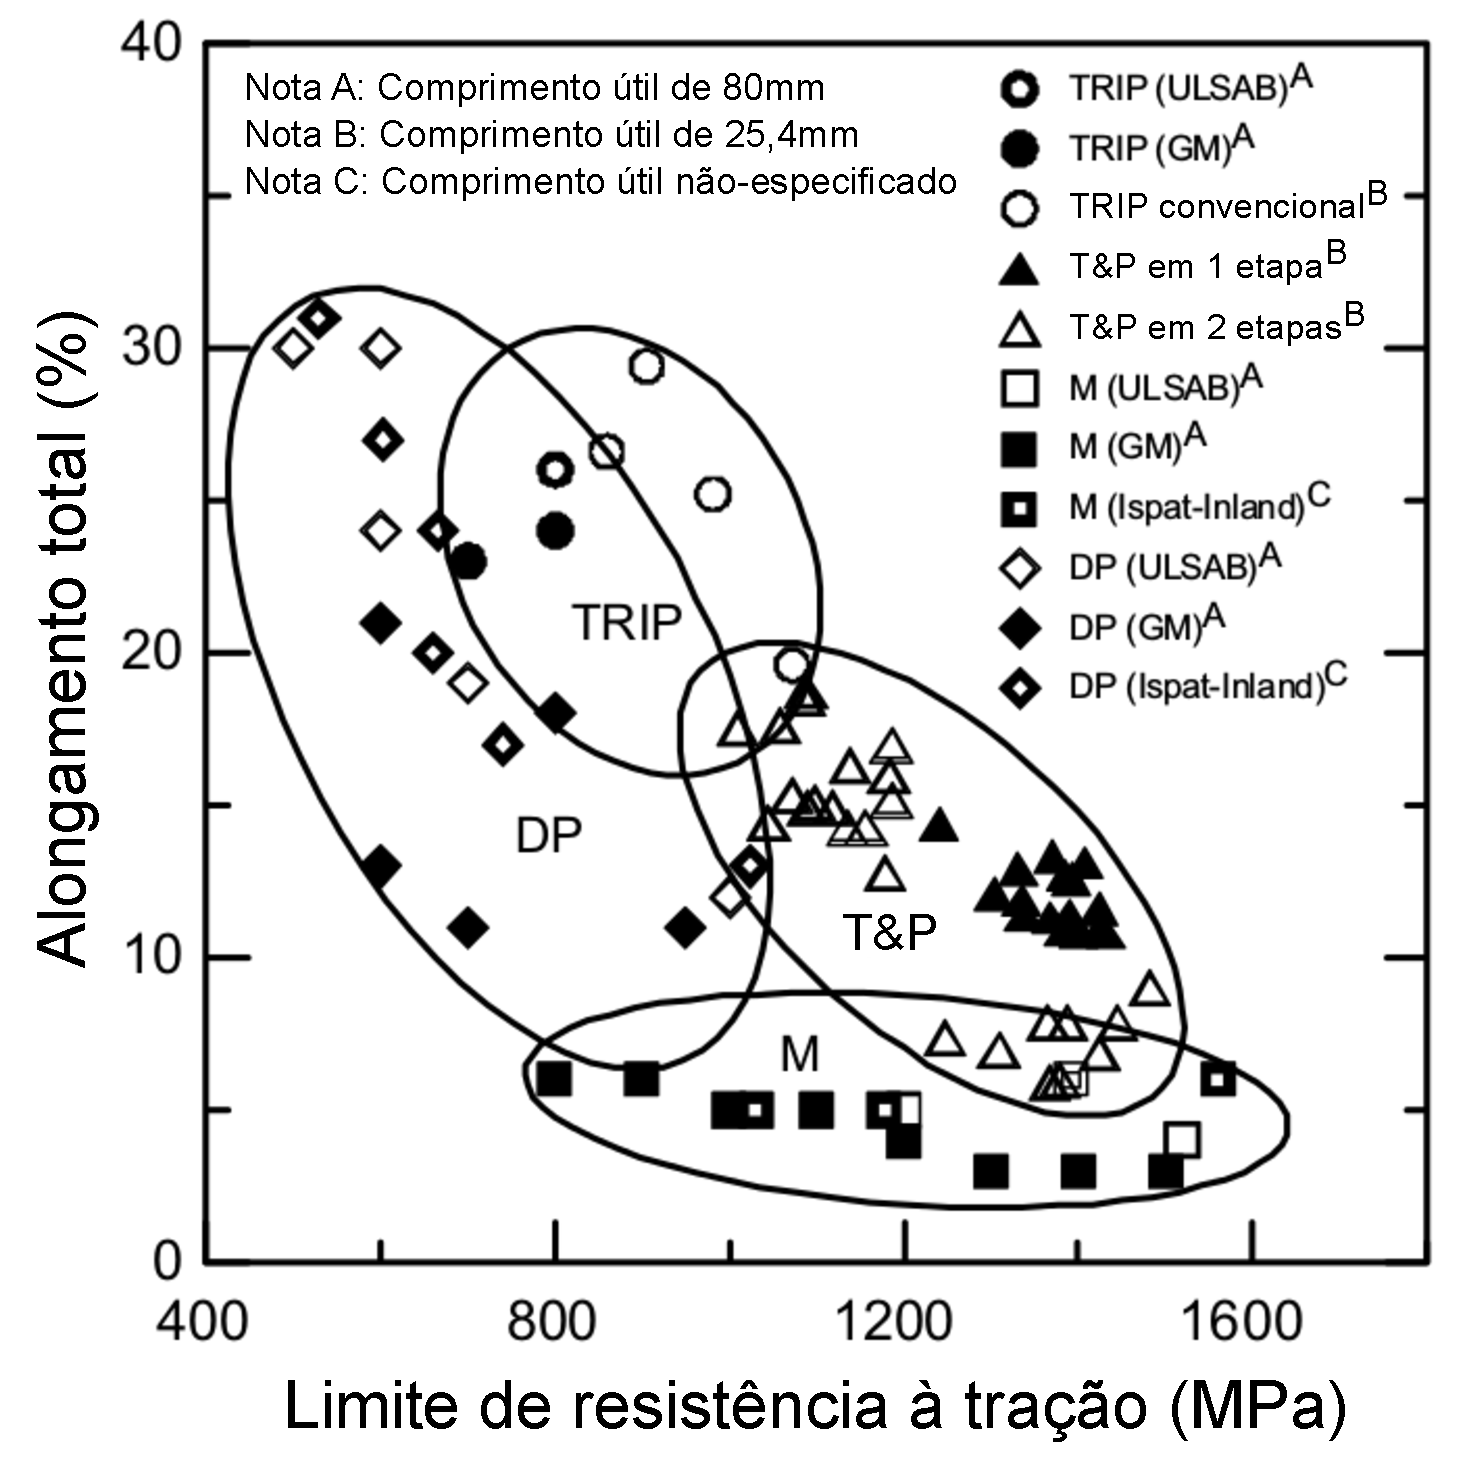
\includegraphics[height=10cm]{img/Streicher.pdf}
	\caption{Alongamento total versus limite de resistência à tração agrupados segundo classes de aços TRIP, \textit{Dual Phase} (DP), martensítico (M) e T\&P tratados em uma ou duas etapas\cite{Streicher2004}.}
	\label{fig:TRIPQP}
\end{figure}

Alinhado ao escopo do presente trabalho, um grupo de estudantes de graduação da \enfase{Colorado School of Mines} examinaram a viabilidade do processo de Têmpera e Partição em um ferro fundido nodular, obtendo quantidade substancial de austenita retida enriquecida em carbono e aumento de resistência mecânica em relação ao ferro fundido nodular austemperado. Entretanto, a quantidade de austenita retida fora menor do que a obtida pelo tratamento de austêmpera, implicando em perda de ductilidade. Os autores comentam que os resultados obtidos foram difíceis de interpretar diante das diferenças entre as frações de fase obtidas durante a têmpera, da precipitação de carbonetos e do comportamento das amostras durante a partição, concluindo que experimentação adicional deve ser realizada para melhor caracterização do fenômeno \cite{Speer2004}.

Inserido do presente grupo de pesquisa, \citaremsentenca{Anderson2013} avaliou a microestrutura e o comportamento mecânico de duas ligas comerciais de ferro fundido com alto manganês (> 0,5\%) tratadas pelo processo T\&P. Silva observou extensas regiões de ausferrita na microestrutura dos materiais tratados termicamente e a ocorrência de uma janela de processo, análoga à precipitação de carbonetos no segundo estágio da reação bainítica no ADI. Os materiais produzidos apresentaram propriedades nos limites da especificação da norma ASTM A897 para ferros fundidos austemperados. Em um trabalho recente, \citaremsentenca{Silva2014} discutiram que as propriedades baixas, ainda que dentro das especificações para ADIs, foram consequência da superposição das janelas de processo das regiões de contorno de célula eutética e próximas aos nódulos. Dessa forma, para incremento das propriedades do ferro fundido T\&P, o teor de manganês haveria de ser diminuído e a inoculação aumenta, minimizando os problemas associados à segregação.

%"O leitor verá que em algumas partes do texto a martensita de baixo carbono é referenciada como ferrita e vice-versa"

\subsection{Termodin\^{a}mica da parti\c{c}\~{a}o de carbono no processo T\&P}

Para compreender as condições termodinâmicas que definem o equilíbrio após o tratamento T\&P, \citaremsentenca{Speer2003} inicialmente assumiram que a redistribuição de carbono entre martensita e austenita ocorreria sem a movimentação da interface. Adicionalmente, como a martensita herda a composição da austenita após a têmpera, a martensita particionada, resultante da relaxação do carbono, deve manter a mesma razão de elementos substitucionais que a austenita. Segundo a definição de Hultgren, portanto, a martensita particionada trata-se essencialmente de paraferrita.

Inicialmente esta condição foi chamada de \enfase{Constrained Paraequilibrium}, ou \sigla{PER}{Paraequilíbrio Restringido}, dada a semelhança com as ideias de Hultgren, com o adendo de que é imposta uma restrição de que os átomos de ferro e substitucionais permanecem \enfase{completamente imóveis} durante a partição de carbono. Dessa forma, a condição proposta prevê que a fração de sítios substitucionais permanece equivalente na austenita e na martensita (equação \ref{eq:potQuimC}) e que a igualdade entre os potenciais químicos de carbono na martensita e na austenita --- ou entre suas atividades, desde que definidas em relação a um estado padrão comum --- também é obedecida (equação \ref{eq:fracSitios}). Entretanto, em troca da imposição de que interface martensita:austenita deve permanecer imóvel, a condição de igualdade dos potenciais químicos do elemento hipotético $Z$, representada pela equação \ref{eq:potQuimZ}, não pode mais ser mantida. Assim, a condição de metaestabilidade é atingida pela minimização da energia livre, dadas as restrições estabelecidas.

Em trabalhos recentes, a condição de paraequilíbrio restringido tem sido referenciada por \enfase{Constrained Carbon Equilibrium}, ou \sigla{ERC}{Equilíbrio Restringido de Carbono}, após discussão realizada entre Speer e colaboradores e Hillert e \AA gren\cite{Hillert2004a,Speer2005,Hillert2005}. \citaremsentenca{Hillert2004a} argumentaram que a relação entre paraequilíbrio e a definição de paraequilíbrio restringido seria mínima, pois: a) paraequilíbrio já se trata de um equilíbrio restringido; b) paraequilíbrio se refere a condições em que ocorre movimentação de interface; c) a redistribuição de elementos substitucionais próximos à interface é praticamente inevitável; d) devido ao requerimento de minimização de energia livre, o PER seria apenas aplicável para o estado final, enquanto a condição de paraequilíbrio se aplica para o crescimento de uma nova fase; e) a redistribuição dos elementos substitucionais para a interface martensita:austenita teria efeito desprezível na redistribuição do carbono entre as duas fases, já que é controlada pelas atividades do carbono. O resultado da equilibração de carbono, portanto, seria independente das condições da interface martensita:austenita.

Em resposta a Hillert e \AA gren, \citaremsentenca{Speer2005} pontuaram que, em essência, o conceito proposto de PER é similar ao de paraequilíbrio, estendido ao ponto de quando a interface permanece imóvel e que não veriam motivo para que houvesse confusão entre as terminologias adotadas. Posteriormente, \citaremsentenca{Hillert2005} reconheceram que a discussão sobre a relação entre paraequilíbrio e PER adquirira características filosóficas e que se tratava, de fato, em aceitar a ampliação do conceito de paraequilíbrio para além de seu campo de aplicação original. Hillert e \AA gren assinalaram que seria desejável preservar o conceito original e sugeriram a utilização do termo \enfase{Constrained Carbon Equilibrium}, apresentado anteriormente. Atualmente esta terminologia parece ter adquirido aceitação geral e vem sendo utilizada desde então\cite{Edmonds2006, Speer2007}. No Brasil, as recentes teses sobre Têmpera e Partição tem adotado a denominação \enfase{Equilíbrio Constrito de Carbono} (ECC)\cite{Martins2007, Coelho2008}. Neste trabalho, a utilização da tradução alternativa Equilíbrio Restringido de Carbono foi adotada por acreditar-se que ela se adéqua melhor à descrição do fenômeno.

\subsubsection{C\'{a}lculo do ERC para ligas Fe-C}

\label{subsubsec:ERC}

O cálculo do ERC em uma determinada liga ferrosa depende de dois principais parâmetros de entrada: a composição química --- em especial, o teor de carbono da liga --- e a fração inicial de austenita não transformada (ou, alternativamente, a fração de martensita)\cite{Speer2003}. Para uma dada condição de austenitização (plena ou parcial), a fração inicial austenita não transformada $f_i^\gamma$ depende da temperatura da têmpera TT aplicada ao material e pode ser estimada pela equação de Koistinen-Marburger (equação \ref{eq:KM}), apresentada anteriormente. Além disso, uma vez que a condição de equilíbrio restringido de carbono impõe uma restrição geométrica ao sistema (imobilidade da interface), o cálculo do ERC requer, além de dados termodinâmicos, obtidos na literatura ou por simulações termodinâmicas, equações secundárias que caracterizam a conservação dos constituintes na microestrutura.

Lobo e Geiger\cite{Lobo1976a,Lobo1976} determinaram as atividades para o carbono na ferrita e na austenita no sistema Fe-C em relação ao estado padrão da grafita.
Para este caso simplificado, é possível ilustrar o problema do cálculo do ERC para um aço carbono. É conveniente, neste caso, expressar os dados na seguinte forma simplificada obtida por \citaremsentenca{Bhadeshia1981}:

\begin{equation}
	RT \ln\frac{\Gamma_C^\alpha}{\Gamma_C^\gamma} = 76789 - 43,8T - (169105 - 120,4) x_C^\gamma
	\label{eq:ativC}
\end{equation}
%
em que $\Gamma^\alpha$ e $\Gamma_C^\gamma$ são respectivamente os coeficientes de atividade Henriana do carbono na ferrita e na austenita, $x_C^\gamma$ é a fração molar de carbono na austenita, $R$ é a contante universal dos gases, equivalente a aproximadamente $8,314 J mol^{-1} K^{-1}$, e $T$ é a temperatura absoluta.

Como a atividade do carbono na fase é calculada pelo produto do coeficiente de atividade pela fração molar de carbono (i.e., $a_C = \Gamma_C x_C$), a condição que leva à equivalência das atividades e dos potenciais químicos do carbono nas duas fases (equação \ref{eq:potQuimC}) é dada pela equação:

\begin{subequations}
	\begin{align}
		x_C^\alpha = x_C^\gamma \exp \left [ - \frac{76789 - 43,8T - (169105 - 120,4T) x_C^\gamma}{RT} \right ]\label{eq:ativC2}
	\end{align}
\end{subequations}
%
em que $x_C^\alpha$ é a fração molar de carbono na ferrita.

As demais equações constitucionais definem o problema por completo:

\begin{subequations}[resume]
	\begin{align}
		&f_{ERC}^\gamma \left ( 1 - x_{C_{ERC}}^\gamma \right ) = f_i^\gamma \left ( 1 - x_{C_i}^\gamma \right )\label{eq:balSubs}\\
		&f_{ERC}^\alpha x_{C_{ERC}}^\alpha + f_{ERC}^\gamma x_{C_{ERC}}^\gamma = x_{C_i}^\gamma\label{eq:balC}\\
		&f_{ERC}^\alpha + f_{ERC}^\gamma = 1\label{eq:balFases}
	\end{align}
\end{subequations}
%
em que $x_{C_i}^\gamma$ é o teor de carbono inicial da austenita, $x_{C_{ERC}}^\alpha$ e $x_{C_{ERC}}^\gamma$ são os teores de carbono na martensita e na austenita na condição de equilíbrio restringido de carbono e $f_{ERC}^\alpha$ e $f_{ERC}^\gamma$ são as frações molares de martensita particionada e austenita na condição de ERC.

A equação \ref{eq:balSubs} estabelece o balanço de massa dos átomos de substitucionais entre a austenita não-transformada inicial e austenita na condição de ERC. É curioso notar que a fração molar da austenita varia dependendo do teor de carbono adquirido após a relaxação de carbono. Essa percepção, inicialmente contraintuitiva, dada a hipótese de interface imóvel, encontra justificativa no fato de que a fração molar da fase depende também da fração de sítios intersticiais ocupados. Assim, variações sutis na fração molar da austenita são oriundas da maior ou menor ocupação dos sítios intersticiais por átomos de carbono.

Por sua vez, a equação \ref{eq:balC} denota um balanço de carbono pela soma ponderada dos teores de carbono na martensita e na austenita. A equação \ref{eq:balFases} estabelece a relação entre as frações de fase, que devem somar a unidade, no caso de austenitização plena, ou um valor menor do que um, equivalente à fração de austenita obtida após o tratamento de austenitização.

A condição de ERC é representada pela solução simultânea das quatro equações \ref{eq:ativC2}--\ref{eq:balFases} para as quatro variáveis desconhecidas $x_{C_{ERC}}^\alpha$, $x_{C_{ERC}}^\gamma$, $f_{ERC}^\alpha$ e $f_{ERC}^\gamma$. A resolução deste sistema não-linear deve ser feita numericamente, pois não apresenta solução analítica.

A formulação descrita acima é estritamente aplicável ao caso do sistema Fe-C, mas pode ser utilizada com considerável fidelidade para aços de baixa liga\cite{Speer2003}. Para que o método adquira caráter rigoroso para as demais ligas, a equação \ref{eq:ativC} deve ser modificada para as atividades do carbono expressas em função dos devidos parâmetros de interação do carbono com os demais elementos de liga. Alternativamente, as atividades do carbono na ferrita e na austenita podem ser determinados utilizando cálculos de termodinâmica computacional.

\subsubsection{Determina\c{c}\~{a}o da temperatura \'{o}tima de t\^{e}mpera}

\label{subsec:tempOtima}

O cálculo do ERC para diferentes temperaturas de têmpera permite a determinação dos parâmetros de tratamento térmico que levam a uma maior retenção de austenita estabilizada por carbono no material. Uma simples metodologia desenvolvida por Speer et al. apud\cite{Edmonds2006} faz uso de equações empíricas para determinação da temperatura Ms (tal qual a equação de Andrews) e da equação de Koistinen-Marburger (equação \ref{eq:KM}) para a computação da fração inicial de austenita não transformada ($f_i^\gamma$) em função da temperatura de têmpera $TT$.

Tendo como parâmetros de entrada $f_i^\gamma$ e o teor de carbono inicial da austenita $x_{C_i}^\gamma$, o ERC é resolvido para uma temperatura de partição $PT$. $PT$ é necessário para o cálculo da relação entre as frações molares de carbono na ferrita e na austenita, expressa pela equação \ref{eq:ativC2}. Por fim, novamente a equação para determinação do Ms e a equação Koistinen-Marburger são aplicadas para o cálculo da quantidade de martensita formada durante o resfriamento final até a temperatura ambiente a partir da austenita não suficientemente estabilizada. Essa martensita é diferente daquela formada após a primeira têmpera, pois ela herda a composição química da austenita enriquecida em carbono durante a partição.

A figura \ref{fig:TPprevisto} ilustra o resultado da predição dos componentes da microestrutura de uma liga hipotética Fe-0,4\%C particionada a 300 °C. É possível perceber que há uma temperatura ótima de têmpera que produz uma fração máxima de austenita retida. Para temperaturas de têmpera superiores à temperatura ótima, há a formação de pequena fração de martensita durante a primeira têmpera, levando a um menor enriquecimento da austenita ao final da etapa partição. Consequentemente, esta austenita não é suficientemente estabilizada e transforma-se parcialmente em martensita durante o resfriamento final.

Para temperaturas menores do que a temperatura ótima, o volume de martensita formado inicialmente é grande e, dessa maneira, há carbono disponível para que toda a austenita não-transformada seja estabilizada durante a partição. A quantidade final de austenita retida ao final do processo, nesse caso, é limitada pela fração de austenita não-transformada durante a têmpera que, como previsto pela equação de Koistinen-Marburger, é tão menor quanto menor a temperatura de têmpera.

\begin{figure}
	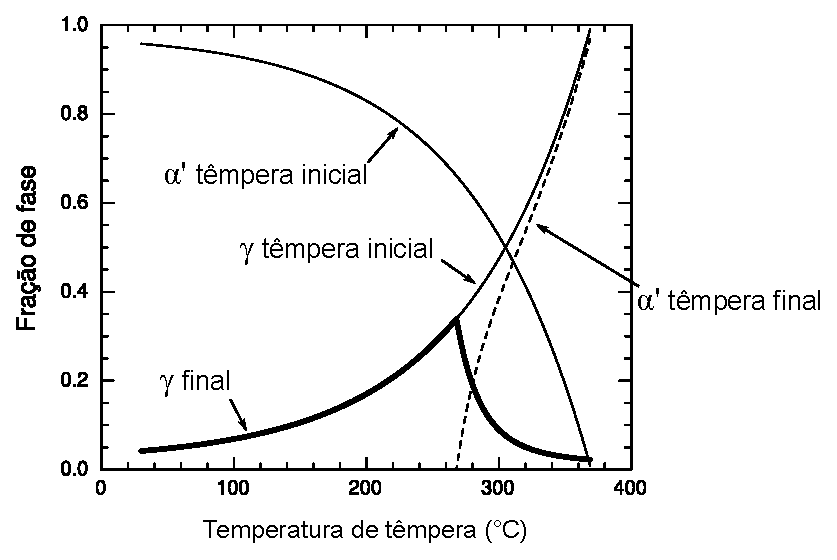
\includegraphics[width=13cm]{img/TPprevisto.pdf}
	\caption{Predição dos componentes da microestrutura de uma liga Fe-0,4\%C particionada a 300°C. A linha sólida espessa representa a fração de austenita ($\gamma$) ao final do processo T\&P. As demais linhas representam a variação das frações de austenita e martensita ($\alpha\text{\textquoteright}$ após a têmpera inicial e a fração de martensita formada no resfriamento final a partir da austenita não suficientemente estabilizada. Curvas recalculadas a partir da metodologia descrita no texto.}
	\label{fig:TPprevisto}
\end{figure}

\subsection{Rea\c{c}\~{o}es competitivas durante o processo T\&P}

\subsubsection{Precipitação de carbonetos}

A precipitação de carbonetos durante a etapa de partição do processo T\&P pode ser interpretada sob o ponto de vista das reações que ocorrem durante o revenimento da martensita. Em baixas temperaturas de revenimento é observada a formação de finas dispersões de carbonetos $\epsilon$, de estrutura hexagonal compacta, e dependendo do teor de carbono, também é possível observar carbonetos de estrutura ortorrômbica $\eta$ e $\chi$. No atual entendimento das reações de revenimento é interpretado que estes carbonetos --- por vezes chamados de carbonetos de transição ou intermediários --- subsequentemente se transformam em precipitados de cementita\cite{Speich1972}. Evitar a precipitação de carbonetos é de fundamental importância para se obter quantidades consideráveis de austenita estabilizada por carbono durante o processo T\&P. Por outro lado, carbonetos de transição não são geralmente considerados prejudiciais para as propriedades mecânicas da martensita revenida, embora a formação de cementita seja aspecto de preocupação\cite{Krauss1983}. Dessa forma, é de particular interesse a compreensão dos parâmetros de tratamento térmico e dos efeitos dos elementos de liga na evolução da precipitação de carbonetos durante o processo T\&P. 

É bem estabelecido que o silício possui um papel importante no retardamento da precipitação da cementita a partir da martensita e da austenita e na transição de carbonetos intermediários para cementita. De fato, este é um dos principais conceitos utilizados no desenvolvimento do processo de Têmpera e Partição. Isto acontece devido à solubilidade desprezível do silício na cementita\cite{Owen1951,Barnard1981a}, implicando que a cinética da precipitação seja controlada pela expulsão do silício da cementita em crescimento para a fase adjacente. Uma vez que as etapas de revenimento/partição se dão normalmente em baixas temperaturas, a reação é lenta.

É possível argumentar que devido à baixa mobilidade do silício, a precipitação de cementita obedeceria condições de paraequilíbrio e, consequentemente, seria muito mais rápida de quando é permitida a redistribuição de substitucionais. No entanto, isto não elimina a evidência experimental de que a precipitação de cementita é retardada na presença de silício. \citaremsentenca{Ghosh2002} estudaram este possível cenário realizando simulações de cinética de precipitação assumindo condições interfaciais de paraquilíbrio. \citaremsentenca{Kozeschnik2008} também exploraram este possível cenário e teorizaram que o crescimento de paracementita estaria associado a uma redução da força motriz para precipitação, consequentemente implicando em uma cinética mais lenta. Os autores mostraram, também por meio de cálculos cinéticos, que isto de fato ocorre para a precipitação da cementita a partir da austenita, embora o modelo tenha falhado em predizer o mesmo fenômeno na precipitação da cementita a partir da ferrita supersaturada em carbono. Os autores justificaram o resultado pelo aprisionamento dos átomos de carbono em defeitos cristalinos na martensita, de modo que o fator controlador da reação seria a eliminação dos defeitos para disponibilização do carbono para formação da cementita.

%Discutir\cite{Caballero2008} por aqui, que fez experimentos de APT em carbonetos formados durante o revenimento de bainita. Resultados deles mostram que não há partição de substitucionais durante os primeiros estágios da formação dos carbonetos. A pergunta é: esses carbonetos são cementita ou na verdade são carbonetos de transição?

Embora o silício seja efetivo no retardamento da precipitação da cementita, o mesmo não pode ser dito sobre seu efeito na precipitação dos carbonetos de transição. \citaremsentenca{Owen1954} e \citaremsentenca{Kenneford1957} mostraram que a cinética do primeiro estágio de revenimento, associada à decomposição da martensita em uma mistura de carbonetos $\epsilon$ e martensita de baixo carbono, é pouco afetada pela presença do silício na liga, enquanto a precipitação de cementita em temperaturas mais elevadas é progressiva e consideravelmente atrasada por adições de silício. \citaremsentenca{Reisdorf1963} mostrou por análises de microsonda eletrônica que durante o revenimento de um aço contendo 0,4\%C e 1,40\%Si que a relação Si:Fe nos carbonetos de revenimento diminui de acordo a transição de carbonetos $\epsilon$ para cementita. Este resultado sinaliza uma maior tolerância dos carbonetos $\epsilon$ ao silício, justificando sua cinética característica. Adicionalmente, a diferença de solubilidades nos carbonetos demanda a partição de silício durante a transição $\epsilon \rightarrow$ cementita.

%Resultados recentes obtidos por tomografia de sonda atômica tridimensional confirmaram este último caso e forneceram informações sobre as condições interfaciais que regem a cinética das reações de precipitação\cite{Zhu2007,Miyamoto2007,Caballero2008}. \citaremsentenca{Miyamoto2007}

%Falar sobre resultados recentes sobre precipitação de carbonetos em materiais temperados e particionados \citaremsentenca{Li2010a} \citaremsentenca{Nayak2008} \citaremsentenca{Edmonds2006}

\subsubsection{Rea\c{c}\~{a}o bainítica e decomposi\c{c}\~{a}o da austenita em temperaturas pr\'{o}ximas \`{a} temperatura Ms}

\label{subsec:decompMs}

A decomposição isotérmica da austenita em temperaturas próximas à temperatura Ms tem sido relatada em uma série de ligas ferrosas. Nestas ligas, uma transformação lenta e isotérmica pode ser observada a baixas temperaturas, ao contrário da cinética rápida, controlada pela nucleação, da martensita atérmica. Diferentes reações são associadas aos produtos formados nesta faixa de temperatura, a citar, a formação de martensita isotérmica a reação bainítica.

A transformação isotérmica da martensita tem sido extensamente estudada em ligas Fe-Ni-Mn em baixas temperaturas\cite{Kaufman1958,Pati1969}. Assim como na formação da martensita atérmica, o crescimento das placas de martensita isotérmica é extremamente rápido, por um mecanismo displacivo, envolvendo uma deformação cisalhante na austenita. Por outro lado, a nucleação deste produto é relativamente lenta, o que permite a determinação das taxas de nucleação envolvidas neste processo\cite{Pati1969}. 

Por sua vez, a observação de martensita isotérmica em ligas contendo carbono é, cinética e microestruturalmente, associada ao estudo da reação bainítica em temperaturas próximas ao Ms. \citaremsentenca{Howard1948} observaram a formação de bainita em temperaturas inferiores ao Ms em ligas Fe-C e Fe-Ni-C, precedida por um tempo de incubação. Os autores reportaram que em uma liga hipereutetóide houve uma mudança anômala na cinética do início da reação em temperaturas ligeiramente acima do Ms, microestruturalmente associada com a formação de um produto em formato de placa finas. \citaremsentenca{Schaaber} determinou por medidas dilatométricas e magnéticas uma reação em dois estágios em temperaturas próximas à temperatura Ms em uma liga Fe-1,16\%C, sugerindo que o primeiro estágio estaria associado à formação de martensita isotérmica, enquanto o estágio subsequente estaria relacionado à reação bainítica.

\citaremsentenca{Radcliffe1959} observaram a ocorrência da aceleração da reação bainítica em temperaturas próximas da temperatura Ms, em ligas hipo e hipereutetóides. Os autores chamaram este fenômeno de \enfase{swing back}. Este fenômeno ocorreria em temperaturas abaixo do Ms em ligas hipoeutetóides e acima do Ms em ligas hipereutetóides. Oka e Okamoto\cite{Okamoto1985,Oka1988} realizaram um estudo sistemático sobre o comportamento da cinética da decomposição da austenita em tratamentos isotérmicos em temperaturas próximas ao Ms em várias ligas Fe-C hipereutetóides, também observando o fenômeno da aceleração da decomposição da austenita nesta faixa de temperaturas. Eles reportaram a observação de um produto em forma de ``finas linhas pretas'' e, mediante análise cristalográfica, concluíram que a fase consistia de martensita formada isotermicamente. Adicionalmente, Oka e Okamoto também concluíram que a presença do produto desempenhara papel na formação de bainita inferior e martensita isotérmica lenticular.

Mais recentemente, \citaremsentenca{VanBohemen2008} reportaram evidências de transformação isotérmica da austenita em temperaturas inferiores ao Ms em aços de baixa liga (Mn e Si) e baixo carbono. Kim e colaboradores\cite{Kim2010,Kim2012} relataram a formação de um produto isotérmico em uma liga de baixo carbono durante o processo de Têmpera e Partição. Foram identificadas diferenças morfológicas, cristalográficas e mecânicas entre os produtos isotérmico e atérmico.

A formação de produtos isotérmicos próximos à temperatura Ms é de crucial importância no entendimento da partição de carbono o processo de têmpera e de partição. \citaremsentenca{Clarke2008} analisaram dois possíveis mecanismos de partição de carbono durante o processo T\&P: (i) partição de carbono da martensita supersaturada para a austenita e (ii) formação de bainita isenta de carbonetos. Eles concluíram que as quantidades de austenita observadas experimentalmente são muito superiores àquelas preditas pelo cálculo teórico considerando a formação de ferrita bainítica e que, portanto, o mecanismo de partição de carbono a partir da martensita é mais consistente com os resultados experimentais. Os autores veem a formação de bainita isenta de carbonetos um mecanismo competitivo no sentido de diminuir a fração de austenita durante a etapa de partição.

%citar o Raabe aqui.

%\bibliography{/home/arthur/Dropbox/Pesquisa/library} % Comentar essa linha antes de compilar versão final.
